% !TeX spellcheck = en_US
\documentclass[AIRbeamer
,optEnglish
%,handout%               deactivate animation
,optBiber
,optBibstyleAlphabetic
,optBeamerClassicFormat% 4:3 format
%,optBeamerWideFormat%   16:9 format
]{AIRlatex}

\usepackage{algorithm}
\usepackage{algorithmicx}

%\setbeameroption{show notes}

\graphicspath{{figures/}}
\addbibresource{source/literature.bib}

\title[Active Tactile Exploration Based on Whisker-Inspired Sensory Array]{Active Tactile Exploration Based on Whisker-Inspired Sensory Array}
\def\PresentationType{\AIRlangGerEng{Abschlussvortrag}{Final Presentation}}
\def\PresentationThesisType{\AIRlangBachelorsThesis}
\author[Valentin Safronov]{Valentin Safronov}
\def\PresentationExaminer{\AIRnamesProfKnoll}
\def\PresentationSupervisor{Yixuan Dang, M.Sc.}
\date{\AIRutilsDate{28}{03}{2025}}

\AIRbeamerSetupHeader{\AIRlayoutHeaderCustomChair}
\AIRbeamerSetupFooterCD

\begin{document}
    \AIRbeamerTitlePageStudentThesis
    \AIRbeamerSetFooterText{\AIRutilsDate{28}{03}{2025}}

    \begin{frame}{Outline}
        \tableofcontents
    \end{frame}


    \section{Introduction}

    \subsection{Whisker Anatomy}
    \begin{frame}{Introduction}{Whisker Anatomy}
        \begin{figure}[htb]
            \centering
            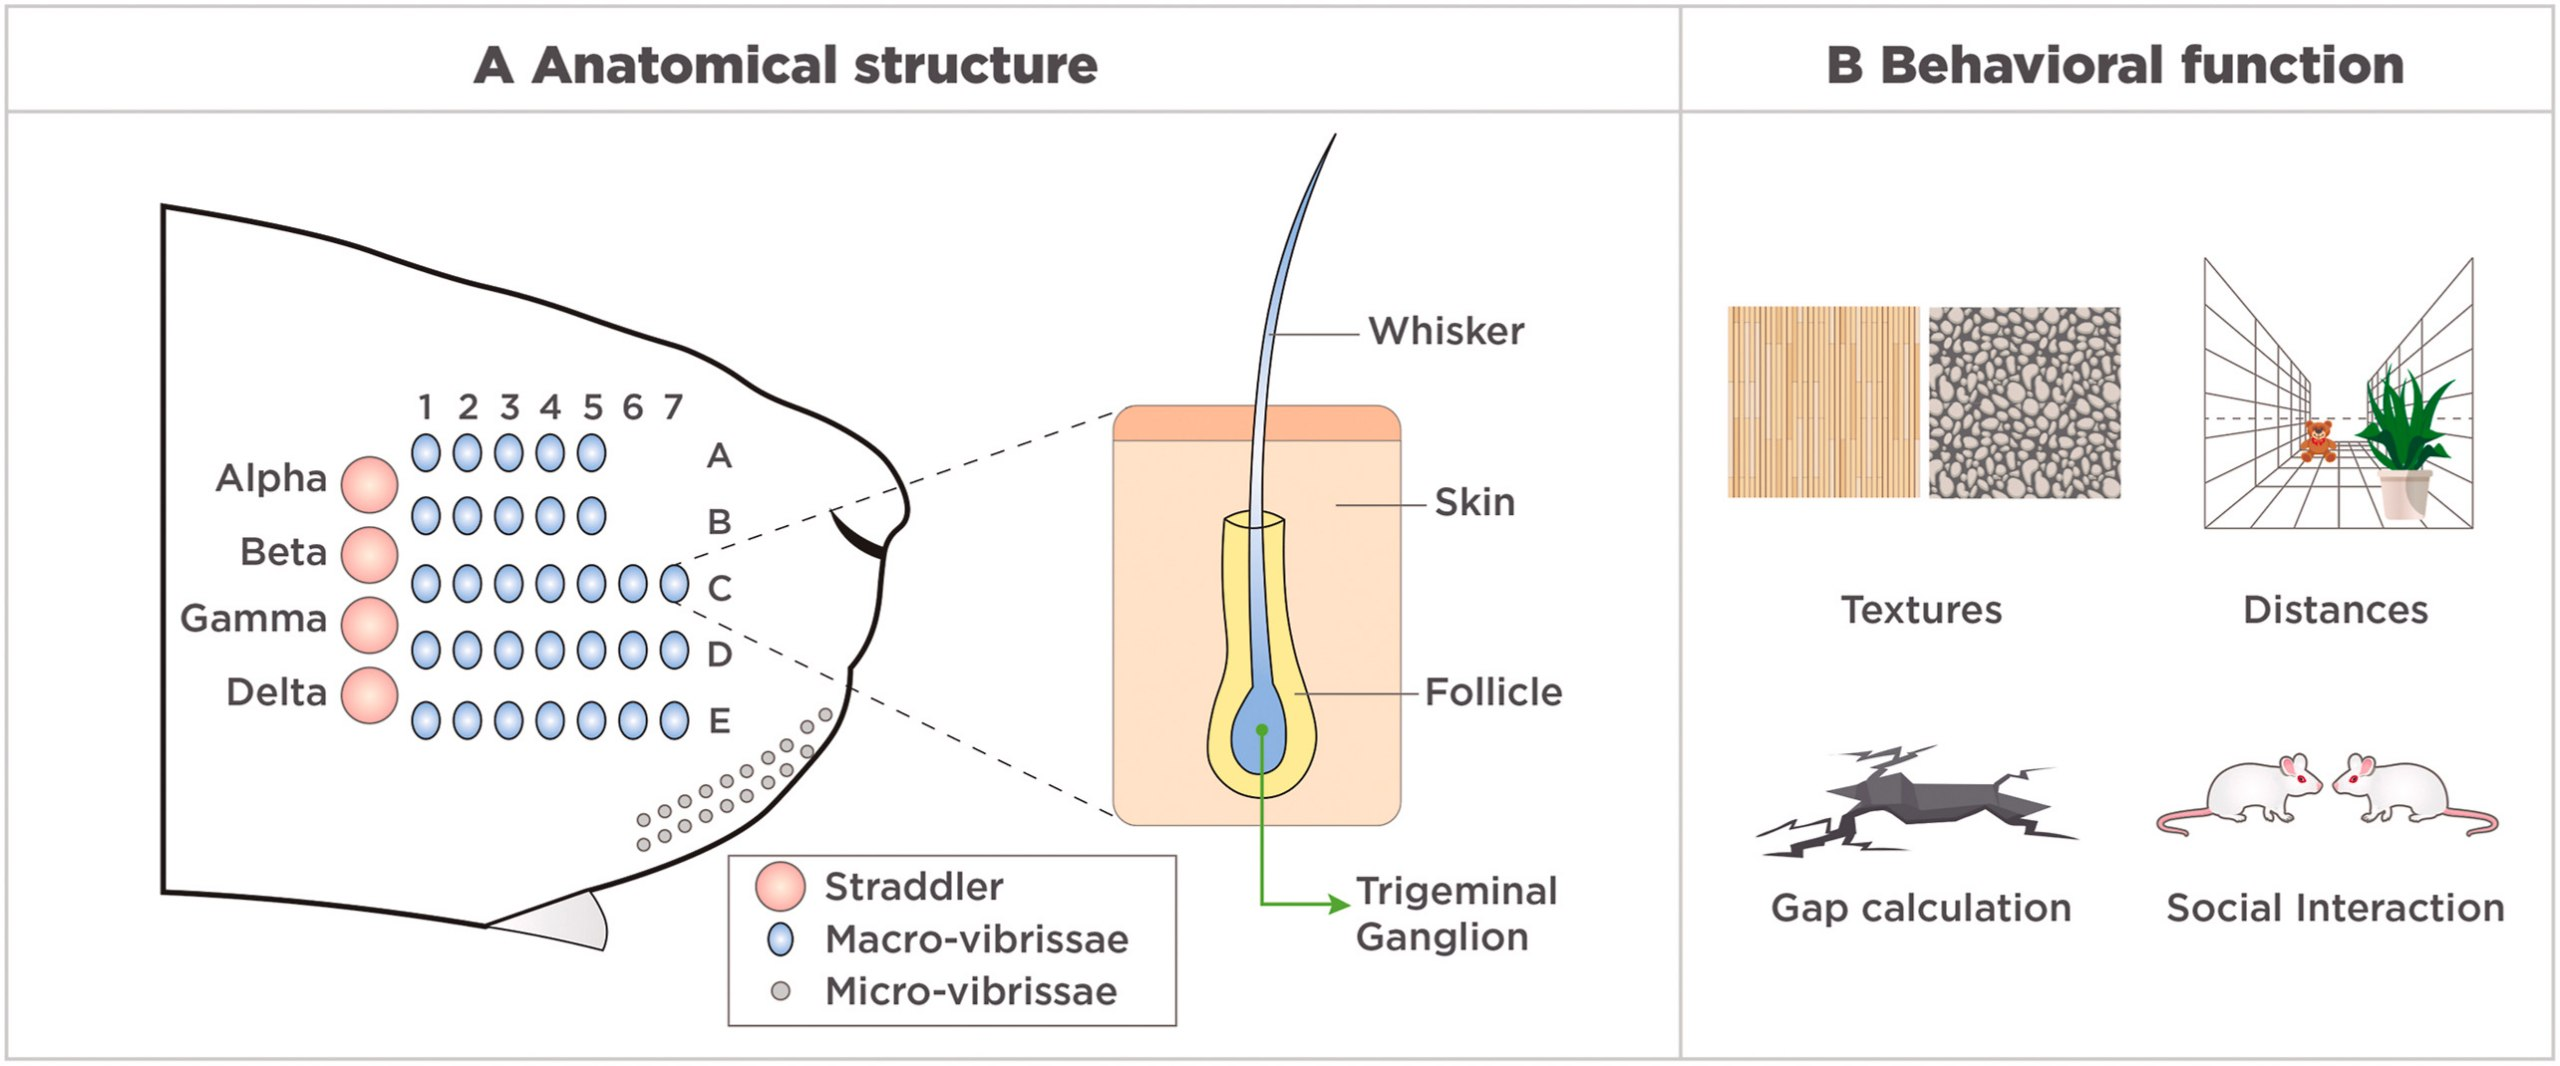
\includegraphics[width=\textwidth]{figures/whisker-anatomy}
            \caption{Representation of the vibrissae system and its function, from~\cite{IBARRACASTANEDA2022100034}}
        \end{figure}
    \end{frame}

    \subsection{Whisker Sensor Applications}
    \begin{frame}{Introduction}{Whisker Sensor Applications}
        Prominent applications according to~\cite{s22072705}:
        \begin{itemize}
            \item Biomimetic tactile: prosthetic feedback via impedance sensing.
            \item Robotic spatial sensing: 3D object localization and environmental mapping.
            \item Surface texture analysis: mapping surface details through whisking data.
            \item Navigation in dark: autonomous whisking for low-light environments.
            \item Underwater sensing: flow detection and vortex vibration control.
        \end{itemize}
    \end{frame}

    \subsection{Robotic Whisker Sensors}
    \begin{frame}[c]{Introduction}{Robotic Whisker Sensors}
        \begin{itemize}
            \item Strain gauge: bending \to strain detection.
            \item Magnetic (Hall): bending \to magnetic shift.
            \item Optical: deflection \to light variation.
        \end{itemize}
        \begin{figure}[H]
            \centering
            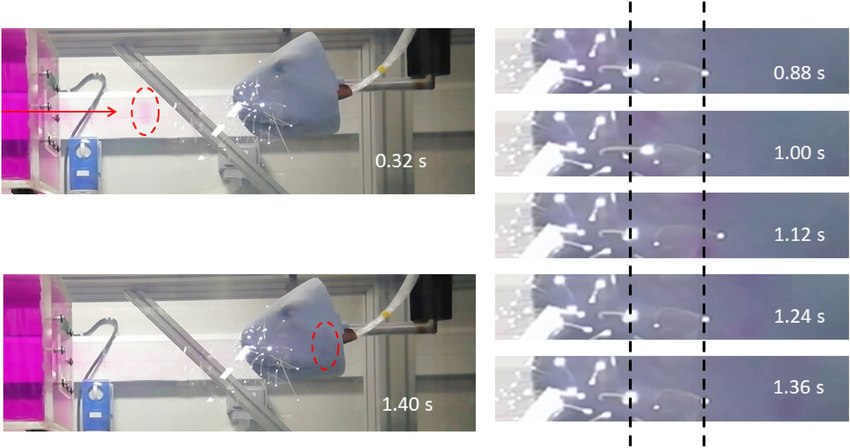
\includegraphics[height=0.5\textheight]{figures/optical-whisker}
            \caption{Picture of the 3D printed sea lion head with integrated optical whiskers, from \cite{optical-whisker}}
        \end{figure}
    \end{frame}

    \subsection{Problem Statement}
    \begin{frame}[c]{Problem Statement}
        \begin{columns}[T,onlytextwidth]
            \begin{column}[T]{0.4\textwidth}
                \only<1-3>{
                    \textbf{Goals:}
                    \begin{itemize}
                        \item Full contour capture
                        \item Precise contour reconstruction
                        \item Navigation in tunnels
                    \end{itemize}
                }
                \only<2-3>{
                    \textbf{Assumptions:}
                    \begin{itemize}
                        \item Navigation and reconstruction in 2D
                        \item Rigid stationary objects
                        \item Contact at the tip
                        \item Known whisker base position
                    \end{itemize}
                }
            \end{column}
            \only<3>{
                \begin{column}[T]{0.2\textwidth}
                    \begin{minipage}[c][.8\textheight][c]{\linewidth}
                        \tikz[baseline=-\baselineskip]\draw[ultra thick,->] (0,0) -- ++ (2,0);
                    \end{minipage}
                \end{column}
                \begin{column}[T]{0.4\textwidth}
                    \begin{minipage}[c][.8\textheight][c]{\linewidth}
                        \textbf{Policies:}
                        \begin{itemize}
                            \item Swiping Policy
                            \item Retrieval Policy
                            \item Tunneling Policy
                            \item Governing Policy
                        \end{itemize}
                    \end{minipage}
                \end{column}
            }
        \end{columns}
    \end{frame}


    \section{Related Work}

    \begin{frame}
        A frame with a magnetic whisker sensor in it.
        \alert{TODO}
    \end{frame}


    \section{Hardware}

    \subsection{Single Whisker Sensor}

    \begin{frame}[c]{Magnetically Transduced Whisker Sensor}
        % TODO: add a magnet picture
        \begin{columns}[c,onlytextwidth]
            \column{0.3\textwidth}
            \centering
            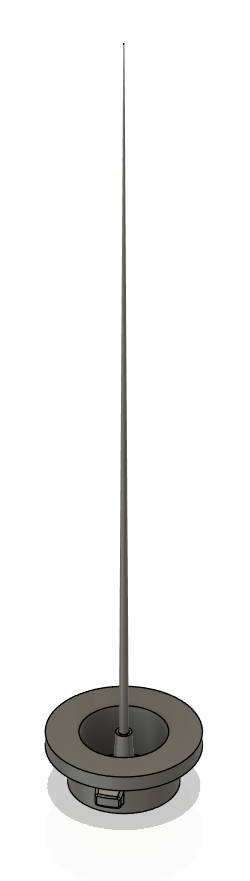
\includegraphics[height=0.6\textheight]{figures/whisker}\\
            (a) Whisker Sensor,\\Whisker shaft -- a nitinol wire
            \column{0.3\textwidth}
            \centering
            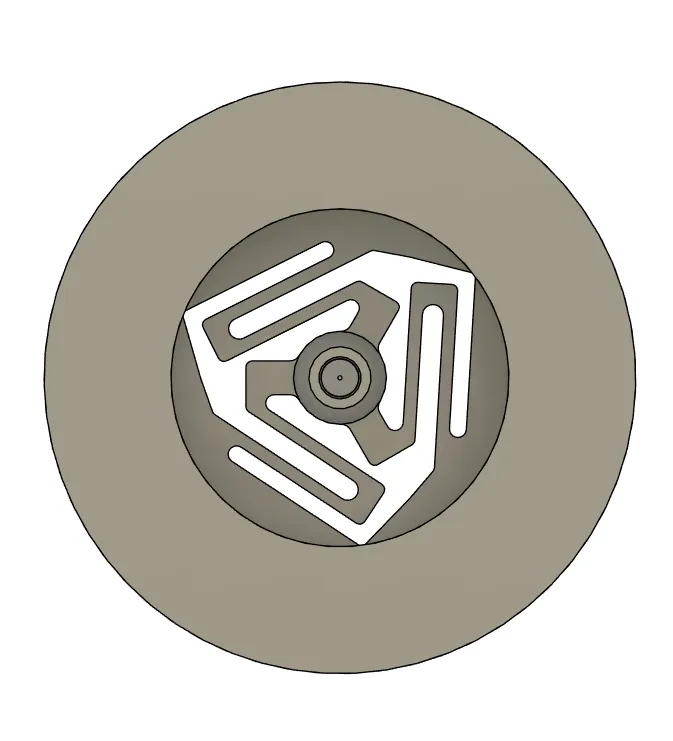
\includegraphics[height=0.6\textheight]{figures/suspension}\\
            (b) Suspension,\\3D-printed with PLA
            \column{0.3\textwidth}
            \centering
            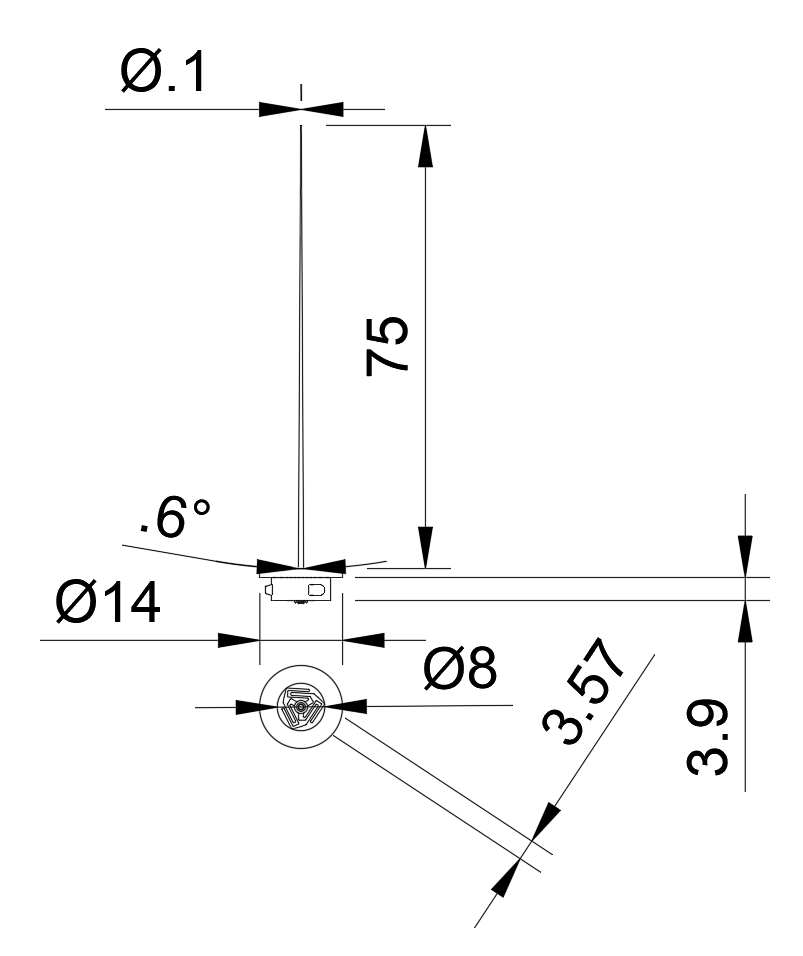
\includegraphics[height=0.6\textheight]{figures/whisker-dims}\\
            (c) Whisker sensor dimensions
        \end{columns}
    \end{frame}

    \note[itemize]{
        \item The whisker shaft is first glued to the suspension system.
        \item A neodymium permanent magnet, axially magnetized with its field direction aligned with the wire, is placed underneath.
        \item The suspension hooks are designed to allow screwing in the whiskers into the whisker mount.
    }

    \begin{frame}{Magnetic Sensor}
        \begin{columns}[T,onlytextwidth]
            \begin{column}[T]{0.6\textwidth}
                \begin{minipage}[c][.8\textheight][c]{\linewidth}
                    \begin{itemize}
                        \item MLX90393 sensor is placed underneath the magnet glued to the suspension.
                        \item Configured for measuring magnetic flux changes with a resolution of \(0.15 \mu T/LSB\).
                        \item The sensor uses I2C communication protocol, acting as a slave.
                        \item If multiple sensors are used, they are connected in a daisy chain.
                    \end{itemize}
                \end{minipage}
            \end{column}
            \begin{column}[T]{0.4\textwidth}
                \begin{figure}[H]
                    \centering
                    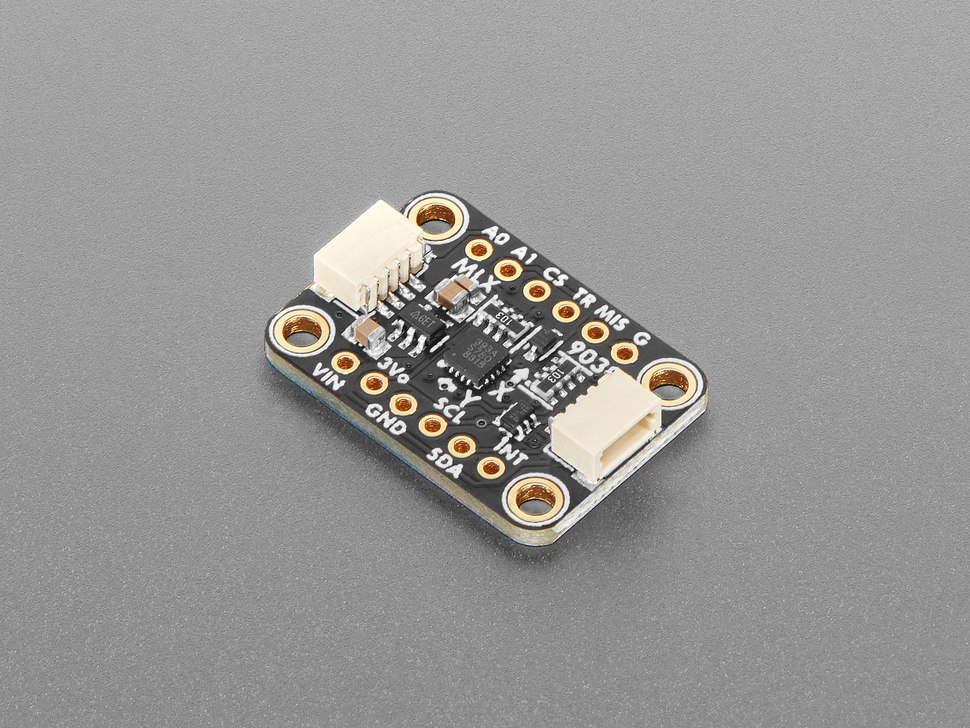
\includegraphics[width=0.7\textwidth]{figures/mlx90393}
                    \caption{Adafruit MLX90393 sensor}
                \end{figure}
                \vskip-0.5cm
                \begin{figure}[H]
                    \centering
                    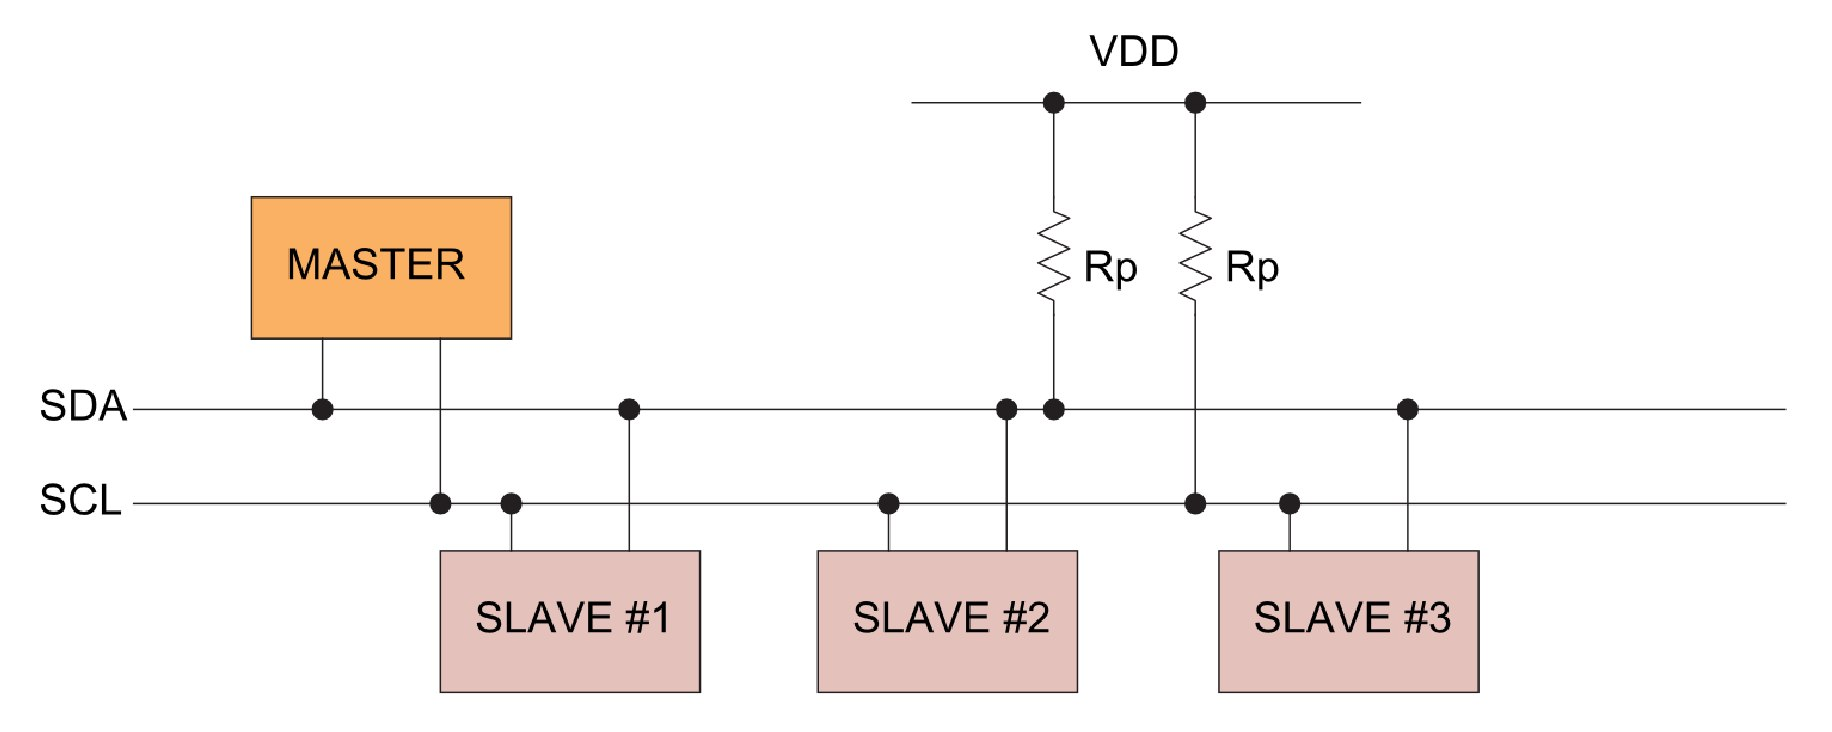
\includegraphics[width=0.7\textwidth]{figures/i2c}
                    \caption{I2C communication}
                \end{figure}
            \end{column}
        \end{columns}
    \end{frame}

    \subsection{Whisker Sensor Array}

    \begin{frame}{Whisker Platform}
        <The CAD drawing of the parts goes here>
        \alert{TODO}

        \begin{figure}[ht]
            \centering
            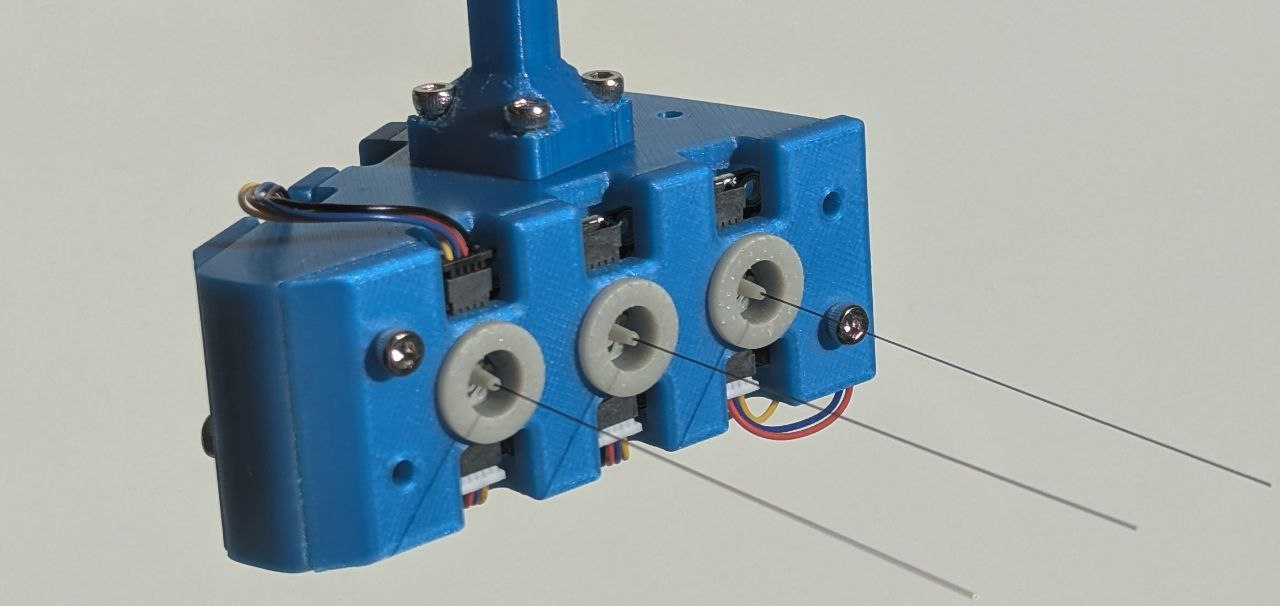
\includegraphics[width=0.6\textheight]{figures/platform}
            \caption{Three whisker attached to the left side and robotic arm mounted at the top}
        \end{figure}
    \end{frame}


    \section{Control Algorithms: Theory and Practice}

    \subsection{Body Motion}
    \begin{frame}{Body Motion}{Control Variables}
        \textbf{Control Inputs:}
        \begin{itemize}
            \item \(^{\mathrm{w}}\boldsymbol{r}^{t}\) -- platform position (world frame).
            \item \(^{\mathrm{w}}\alpha^{t}\) -- platform orientation (world frame).
            \item \(\delta_{\mathrm{wsk,i}}^{t}\) -- deflection of the whiskers for i
        \end{itemize}

        \textbf{Control Outputs:}
        \begin{itemize}
            \item \(^{\mathrm{w}}\boldsymbol{v}^{t}\) -- platform velocity (world frame).
            \item \(^{\mathrm{w}}\omega^{t}\) -- platform angular velocity (world frame).
        \end{itemize}
    \end{frame}

    \begin{frame}{Body Motion}{Control Algorithm}
        \begin{algorithm}[H]
            \caption{Steer the Platform to Target Position and Orientation}
            \begin{algorithmic}[1]
                \State Require \(^{\mathrm{w}}\boldsymbol{r}^{t+1}\), \(\;^{\mathrm{w}}\alpha^{t+1}\)
                \State \(^{\mathrm{w}}\omega^{t+1} \gets \mathrm{PID}(\;^{\mathrm{w}}\alpha^{t+1} - \;^{\mathrm{w}}\alpha^{t})\)
                \State \(^{\mathrm{w}}\boldsymbol{v}^{t+1} \gets v_{\mathrm{total}} \cdot \dfrac{\;^{\mathrm{w}}\boldsymbol{r}^{t+1} - \;^{\mathrm{w}}\boldsymbol{r}^{t}}{\|^{\mathrm{w}}\boldsymbol{r}^{t+1} - \;^{\mathrm{w}}\boldsymbol{r}^{t}\|}\)
                \State Return \(^{\mathrm{w}}\boldsymbol{v}^{t+1}\), \(^{\mathrm{w}}\omega^{t+1}\)
            \end{algorithmic}
            \label{alg:steer_platform}
        \end{algorithm}

        \begin{algorithm}[H]
            \caption{Steer Whisker to Target Position and Orientation}
            \begin{algorithmic}[1]
                \State Require \(^{\mathrm{w}}\boldsymbol{r}_{\mathrm{wsk}}^{t+1}\), \(^{\mathrm{w}}\alpha_{\mathrm{wsk}}^{t+1}\)
                \State \((^{\mathrm{w}}\boldsymbol{v}^{t+1},\, ^{\mathrm{w}}\omega^{t+1}) \gets \mathrm{steer\_body}(\;^{\mathrm{w}}\boldsymbol{r}_{\mathrm{wsk}}^{t+1},\, ^{\mathrm{w}}\alpha_{\mathrm{wsk}}^{t+1})\)
                \State \(^{\mathrm{w}}\boldsymbol{r}_{\mathrm{corr}} \gets [0,\,0,\,^{\mathrm{w}}\omega^{t+1}] \times \boldsymbol{r}_{\mathrm{wsk, body}}\)
                \State \(^{\mathrm{w}}\boldsymbol{v}^{t+1} \gets v_{\mathrm{total}} \cdot \dfrac{^{\mathrm{w}}\boldsymbol{v}^{t+1} + \,^{\mathrm{w}}\boldsymbol{r}_{\mathrm{corr}}}{\|^{\mathrm{w}}\boldsymbol{v}^{t+1} + \,^{\mathrm{w}}\boldsymbol{r}_{\mathrm{corr}}\|}\)
                \State Return \(^{\mathrm{w}}\boldsymbol{v}^{t+1}\), \(^{\mathrm{w}}\omega^{t+1}\)
            \end{algorithmic}
            \label{alg:steer_whisker}
        \end{algorithm}

    \end{frame}

    \subsection{Swiping Policy}
    \begin{frame}{Swiping Policy}{Control Algorithm}
        \begin{algorithm}[H]
            \caption{Swiping Policy}
            \begin{algorithmic}[1]
                \only<1>
                {
                    \State If \(|\delta_{\mathrm{wsk}}^{t}| < \delta_{\mathrm{wsk, thr}}\)
                    Then
                    \State \quad Return \(\;^{\mathrm{w}}\boldsymbol{v}^{t}\), \(\;^{\mathrm{w}}\omega^{t}\)
                    \State End If
                    \State
                    \State \(\;^{\mathrm{s}}\boldsymbol{r}_{\mathrm{tip}}^{t} \gets \mathrm{wsk.defl\_model}(\delta_{\mathrm{wsk}}^{t})\)
                    \State \(\;^{\mathrm{w}}\boldsymbol{r}_{\mathrm{tip}}^{t} \gets \;^{\mathrm{w}}\boldsymbol{r}^{t} + \;^{\mathrm{w}}\boldsymbol{r}_{\mathrm{wsk, body}} + \boldsymbol{R}_{xy}^{2}(\; ^{\mathrm{w}}\alpha_{\mathrm{wsk}}^{t}) \cdot \;^{\mathrm{s}}\boldsymbol{r}_{\mathrm{tip}}^{t}\)
                    \State \colorbox{yellow!40}{\(\mathrm{wsk.spline.add\_keypoint}(\;^{\mathrm{w}}\boldsymbol{r}_{\mathrm{tip}}^{t})\)}
                    \State If not \(\mathrm{wsk.spline.has\_enough\_points()}\)
                    Then
                    \State \quad Return \(\;^{\mathrm{w}}\boldsymbol{v}^{t}\), \(\;^{\mathrm{w}}\omega^{t}\)
                    \State End If
                }
                \only<2>
                {
                    \setcounter{ALG@line}{10}
                    \State \(\;^{\mathrm{w}}\boldsymbol{\tau}_{\mathrm{spline}}^{t} \gets \dfrac{\mathrm{wsk.spline}(u\mathord{=}u_{k1}) - \mathrm{wsk.spline}(u\mathord{=}u_{k0})}{\|\mathrm{wsk.spline}(u\mathord{=}u_{k1}) - \mathrm{wsk.spline}(u\mathord{=}u_{k0})\|}\)
                    \State \colorbox{cyan!40}{\(\;^{\mathrm{w}}\theta_{\mathrm{spline}}^{t} \gets \mathrm{arctan2}(\;^{\mathrm{w}}\boldsymbol{\tau}_{\mathrm{spline}}^{t})\)}
                    \State \(\;^{\mathrm{s}}\boldsymbol{r}_{\mathrm{tip, target}}^{t} \gets \mathrm{wsk.defl\_model}\big(\delta_{\mathrm{wsk, target}} \cdot \operatorname{sgn}(\delta_{\mathrm{wsk}}^{t})\big)\)
                    \State \(\Delta\boldsymbol{r}_{tip}^{t} \gets \boldsymbol{R}_{xy}^{2}(\; ^{\mathrm{w}}\alpha_{\mathrm{wsk}}^{t}) \cdot (\;^{\mathrm{s}}\boldsymbol{r}_{\mathrm{tip, target}}^{t} - \;^{\mathrm{s}}\boldsymbol{r}_{\mathrm{tip}}^{t})\)
                    \State \(\;^{\mathrm{s}}\boldsymbol{r}_{\mathrm{tip, neutral}} \gets \mathrm{wsk.defl\_model}(0)\)
                    \State \(w_{\mathrm{defl}}^{t} \gets \dfrac{\|\Delta\boldsymbol{r}_{\mathrm{tip}}^{t}\|}{\|\;^{\mathrm{s}}\boldsymbol{r}_{\mathrm{tip, target}}^{t} - \;^{\mathrm{s}}\boldsymbol{r}_{\mathrm{tip, neutral}}\|}\)
                    \State \colorbox{green!40}{\(\;^{\mathrm{w}}\boldsymbol{r}_{\mathrm{wsk}}^{t+1} \gets \;^{\mathrm{w}}\boldsymbol{r}_{\mathrm{wsk}}^{t} + w_{\mathrm{defl}}^{t} \cdot \dfrac{-\Delta\boldsymbol{r}_{\mathrm{tip}}^{t}}{\|\Delta\boldsymbol{r}_{\mathrm{tip}}^{t}\|} + (1 - w_{\mathrm{defl}}^{t}) \cdot \dfrac{\;^{\mathrm{w}}\boldsymbol{\tau}_{\mathrm{spline}}^{t}}{\|\;^{\mathrm{w}}\boldsymbol{\tau}_{\mathrm{spline}}^{t}\|}\)}
                    \State \((\;^{\mathrm{w}}\boldsymbol{v}^{t+1}, \;^{\mathrm{w}}\omega^{t+1}) \gets \mathrm{steer\_wsk}(\;^{\mathrm{w}}\boldsymbol{r}_{\mathrm{wsk}}^{t+1},\;^{\mathrm{w}}\theta_{\mathrm{spline}}^{t})\)
                    \State Return \(\;^{\mathrm{w}}\boldsymbol{v}^{t+1}, \;^{\mathrm{w}}\omega^{t+1}\)
                }
            \end{algorithmic}
        \end{algorithm}
    \end{frame}
    \begin{frame}{Swiping Policy}{Simulation Results}
        \begin{figure}[htb]
            \centering
            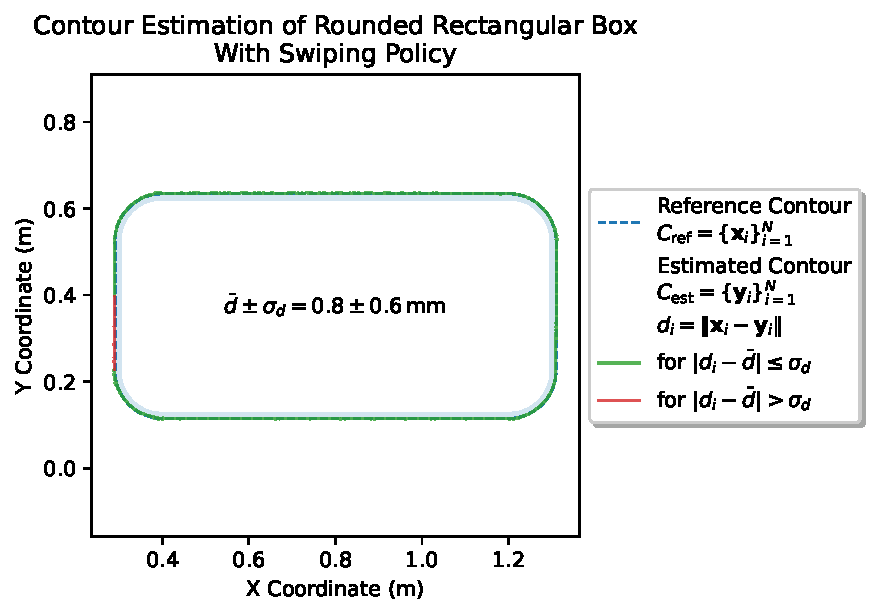
\includegraphics[width=0.7\textwidth]{figures/experiments/rounded-rectangular-box-swiping}
        \end{figure}
    \end{frame}
    \begin{frame}{Swiping Policy}{Simulation Results}
        \begin{figure}[htb]
            \centering
            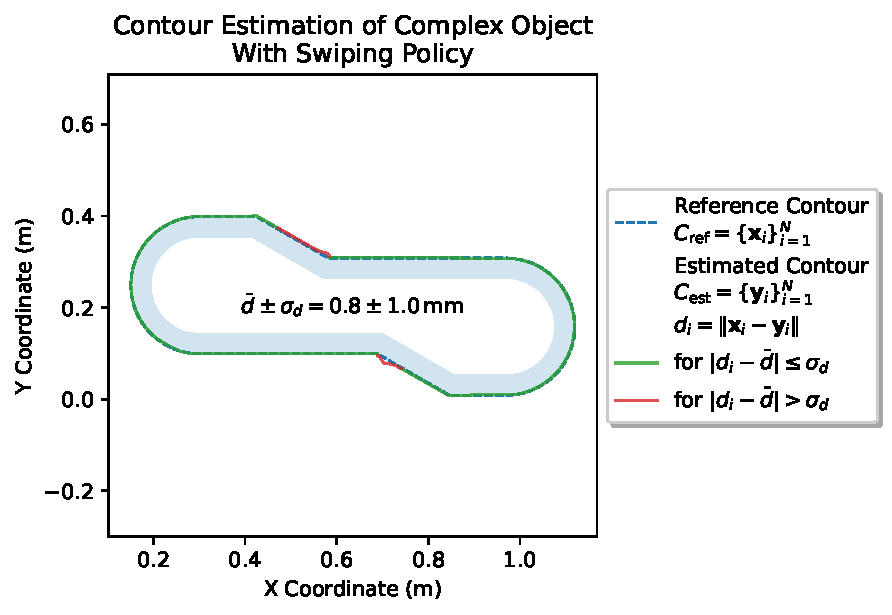
\includegraphics[width=0.7\textwidth]{figures/experiments/complex-object-swiping}
        \end{figure}
    \end{frame}

    \subsection{Retrieval Policy}
    \begin{frame}[c]{Retrieval Policy}{Motivation}
        \begin{columns}[T,onlytextwidth]
            \begin{column}[T]{0.48\textwidth}
                \begin{figure}[H]
                    \centering
                    \captionsetup{justification=centering}
                    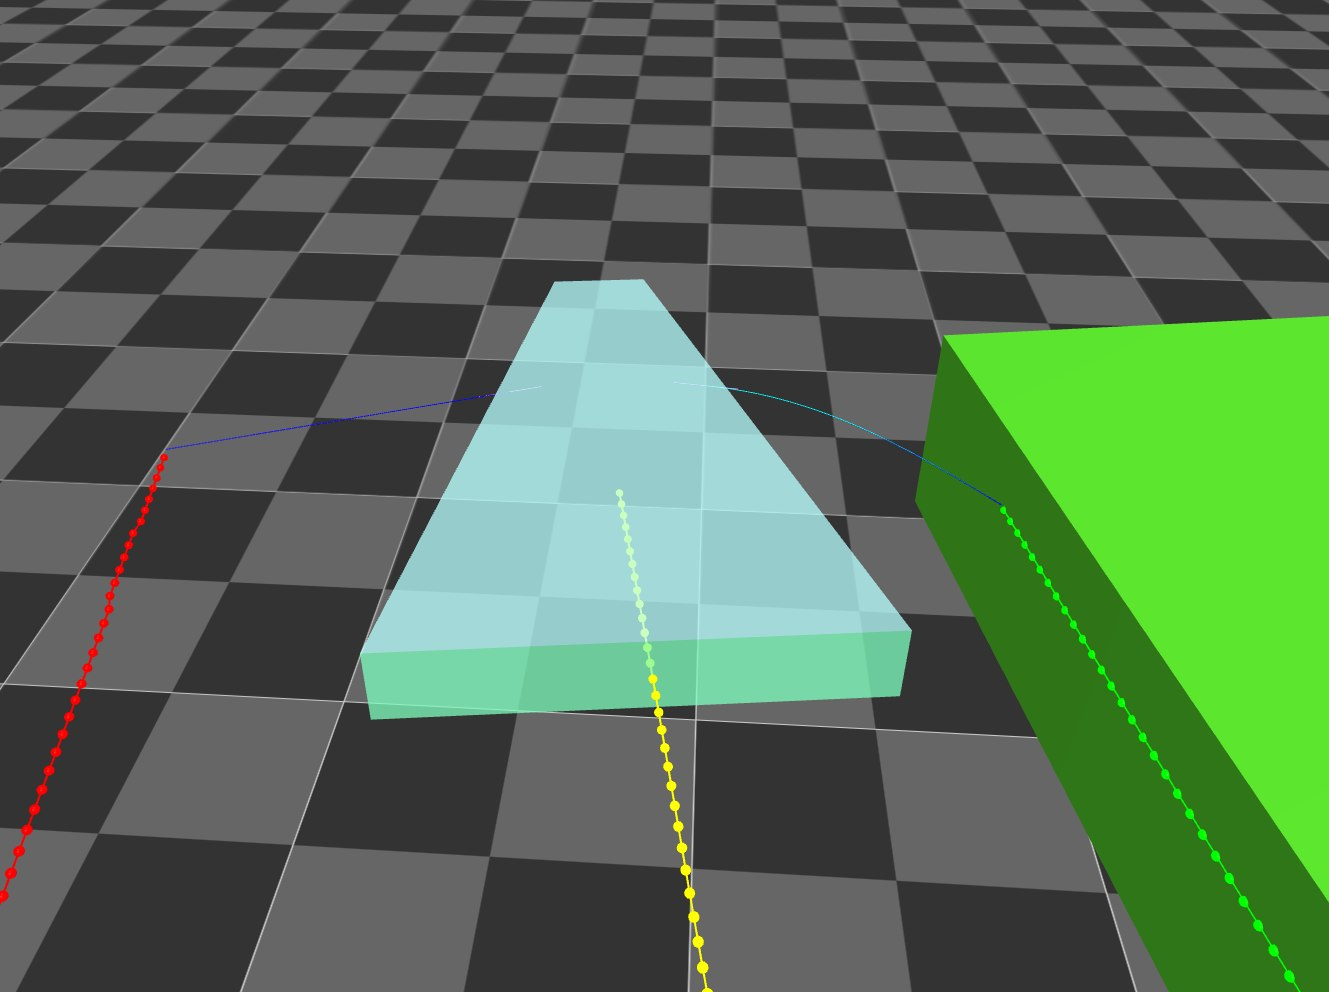
\includegraphics[width=\textwidth]{figures/retrieval/before}
                    \caption{\textbf{(0.1) Initial situation}\\Swiping along the side of the object.}
                \end{figure}
            \end{column}
            \begin{column}[T]{0.48\textwidth}
                \begin{figure}[H]
                    \centering
                    \captionsetup{justification=centering}
                    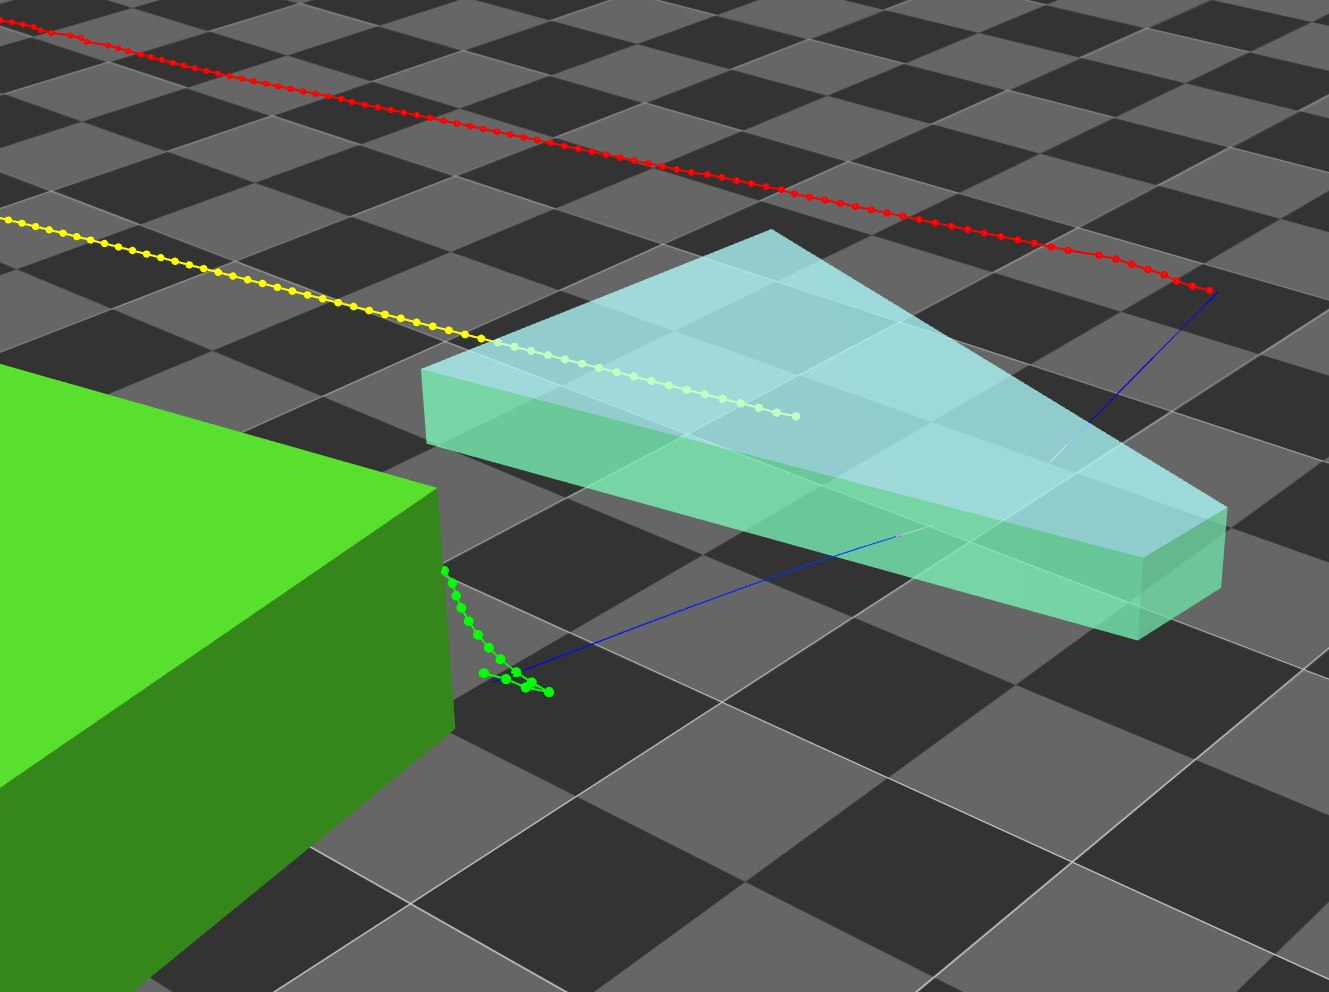
\includegraphics[width=\textwidth]{figures/retrieval/disengagement}
                    \caption{\textbf{(0.2) Disengagement}\\Whisker has detached.}
                \end{figure}
            \end{column}
        \end{columns}
    \end{frame}
    \begin{frame}[c]{Retrieval Policy}{Angle Resolution}
        \begin{columns}[T,onlytextwidth]
            \begin{column}[T]{0.48\textwidth}
                \begin{minipage}[c][.8\textheight][c]{\linewidth}
                    \begin{enumerate}
                        \item \textbf{Angle Resolution}
                        \begin{enumerate}
                            \item Construct a circle of potential contact points
                            \item Move to the first candidate point
                            \item Move sequentially from one candidate point to another until the contact is established
                            \item Calculate the edge angle
                        \end{enumerate}
                    \end{enumerate}
                \end{minipage}
            \end{column}
            \begin{column}[T]{0.48\textwidth}
                \begin{figure}[H]
                    \centering
                    \begin{tikzpicture}[scale=2]
                        \coordinate (E) at (0,0);
                        \coordinate (X) at (2,0);
                        \coordinate (Y) at ({2*cos(30)},{2*sin(30)});
                        \coordinate (Yp) at ({2*cos(135)},{2*sin(135)});
                        \coordinate (C) at ({cos(30)},{sin(30)});
                        \coordinate (W) at ({cos(135)}, {sin(135)});
                        \coordinate (T) at ({cos(135) - cos(135 - 90)}, {sin(135) - sin(135 - 90)});
                        \coordinate (B) at ({cos(135) - 2*cos(135 - 90 + 20)}, {sin(135) - 2*sin(135 - 90 + 20)});

                        \draw [blue, dotted] (E) circle (1);
                        \draw (E) -- (X);
                        \draw (E) -- (Y);
                        \draw [green] (B) -- (W);
                        \draw [blue, dashed] (E) -- (Yp);
                        \draw [blue, dashed] (W) -- (T);

                        % Mark the 30° angle at vertex B.
                        \draw (0.5,0) arc (0:30:0.5);
                        \node at (0.8,0.15) {$\beta$};

                        % Label the points.
                        \fill (X) circle (1pt) node[below right] {$X$};
                        \fill (E) circle (1pt) node[below left] {$E$};
                        \fill (Y) circle (1pt) node[above right] {$Y$};
                        \fill (Yp) circle (1pt) node[above right] {$Y'$};
                        \fill (W) circle (1pt) node[above left] {$W$};
                        \fill (B) circle (1pt) node[above left] {$B$};
                        \fill (T) circle (1pt) node[above left] {$T$};

                    \end{tikzpicture}
                    \caption{Angle Resolution at Edge E \\Black $[XE]$, $[EY]$ \textemdash{} object surface,\\Green $[BW]$ \textemdash{} the whisker,\\Blue $[EY']$ \textemdash{} the potential adjacent surface of the edge and its tangent $[WT]$,\\Blue circle \textemdash{} the targeted contact points.}
                \end{figure}
            \end{column}
        \end{columns}
    \end{frame}
    \begin{frame}[c]{Retrieval Policy}{Angle Resolution}
        \begin{columns}[T,onlytextwidth]
            \begin{column}[T]{0.48\textwidth}
                \begin{figure}[H]
                    \centering
                    \captionsetup{justification=centering}
                    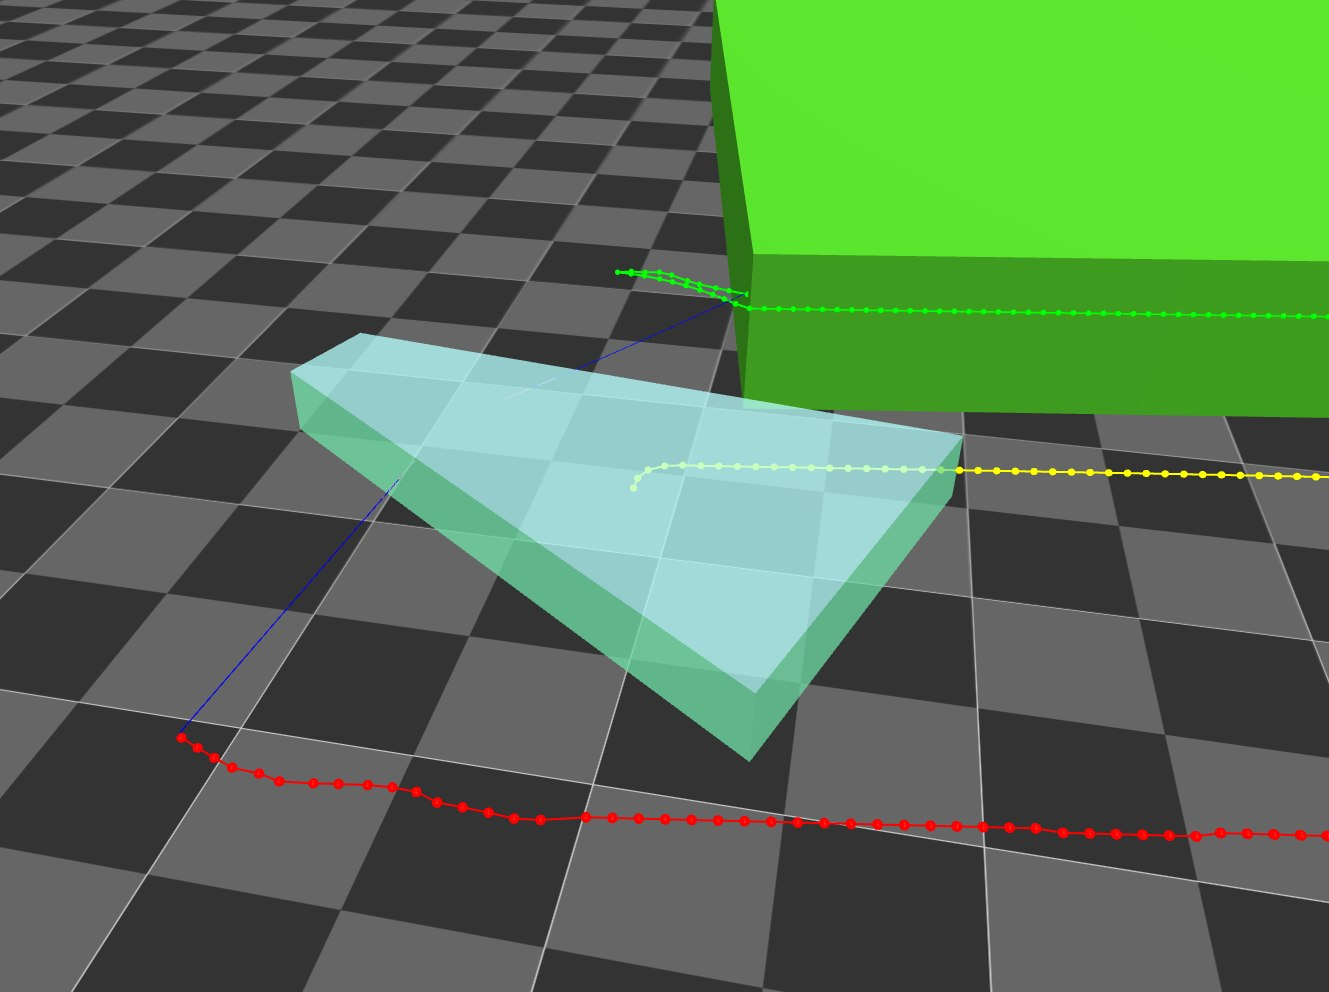
\includegraphics[width=\textwidth]{figures/retrieval/retrieval}
                    \caption{\textbf{\alert{TODO} (1.1) Retrieval}\\Whisker has retrieved the contact.}
                \end{figure}

            \end{column}
            \begin{column}[T]{0.48\textwidth}
                \begin{figure}[H]
                    \centering
                    \captionsetup{justification=centering}
                    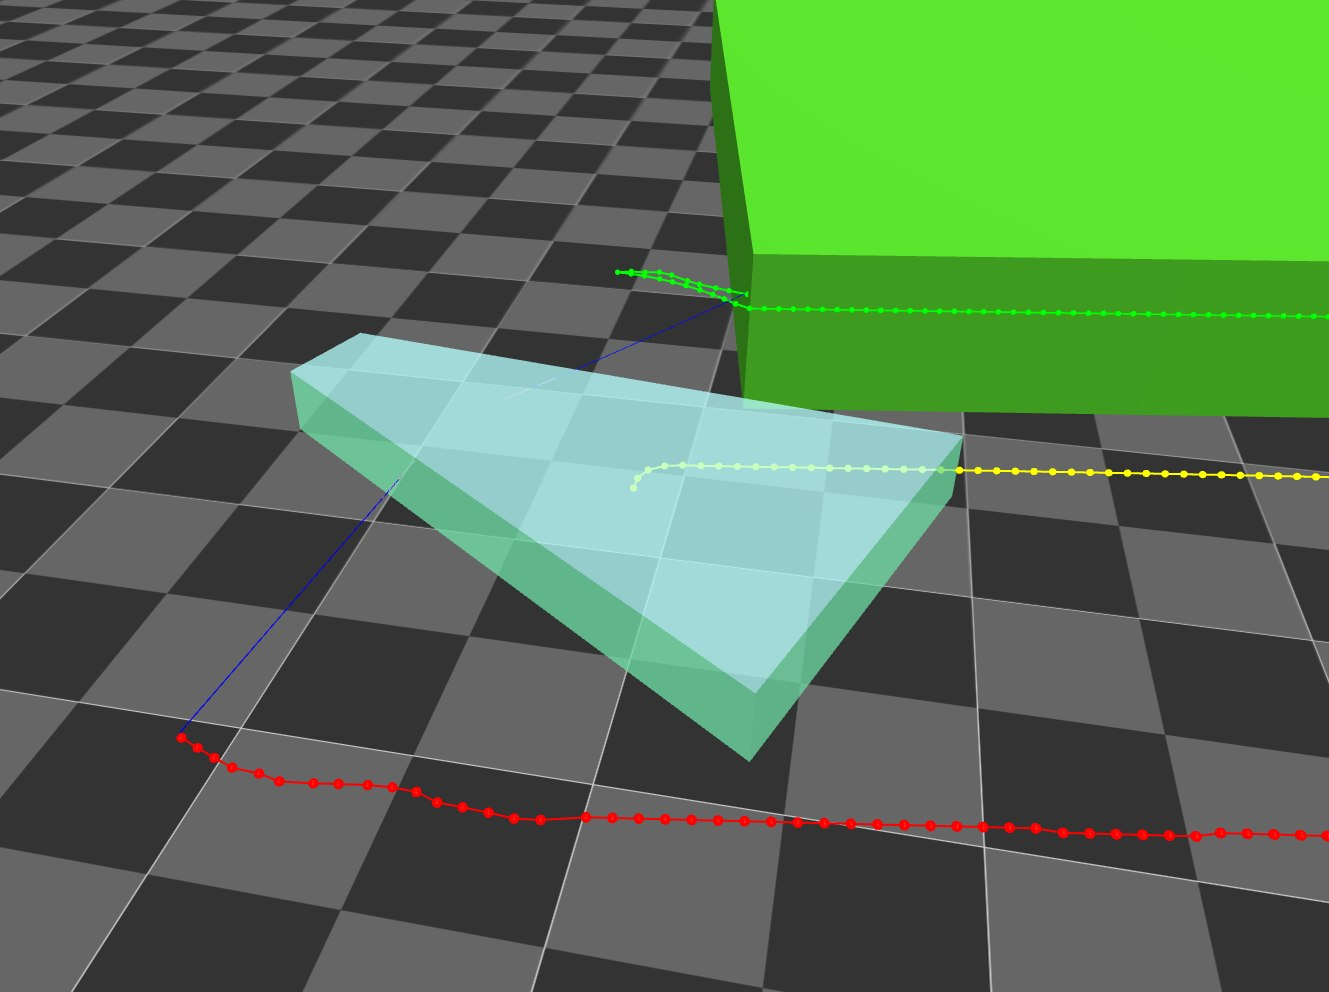
\includegraphics[width=\textwidth]{figures/retrieval/retrieval}
                    \caption{\textbf{(1.2) Retrieval}\\Whisker has retrieved the contact.}
                \end{figure}
            \end{column}
        \end{columns}
    \end{frame}
    \begin{frame}[c]{Retrieval Policy}{Whisking and Transition to Swiping}
        \begin{enumerate}
            \setcounter{enumi}{1}
            \item \textbf{Whisking Back to the Edge}
            \begin{enumerate}
                \item Move back along the opposite side of the edge
                \item Disengage the whisker at the edge
            \end{enumerate}
            \item \textbf{Transition to Swiping}
            \begin{enumerate}
                \item Reposition the whisker with a slight overshoot
                \item Move towards the object until the contact is re-established
                \item Transfer control to the exploration policy
            \end{enumerate}
        \end{enumerate}
    \end{frame}
    \begin{frame}[c]{Retrieval Policy}{Whisking and Repositioning}
        \begin{columns}[T,onlytextwidth]
            \begin{column}[T]{0.48\textwidth}
                \begin{figure}[H]
                    \centering
                    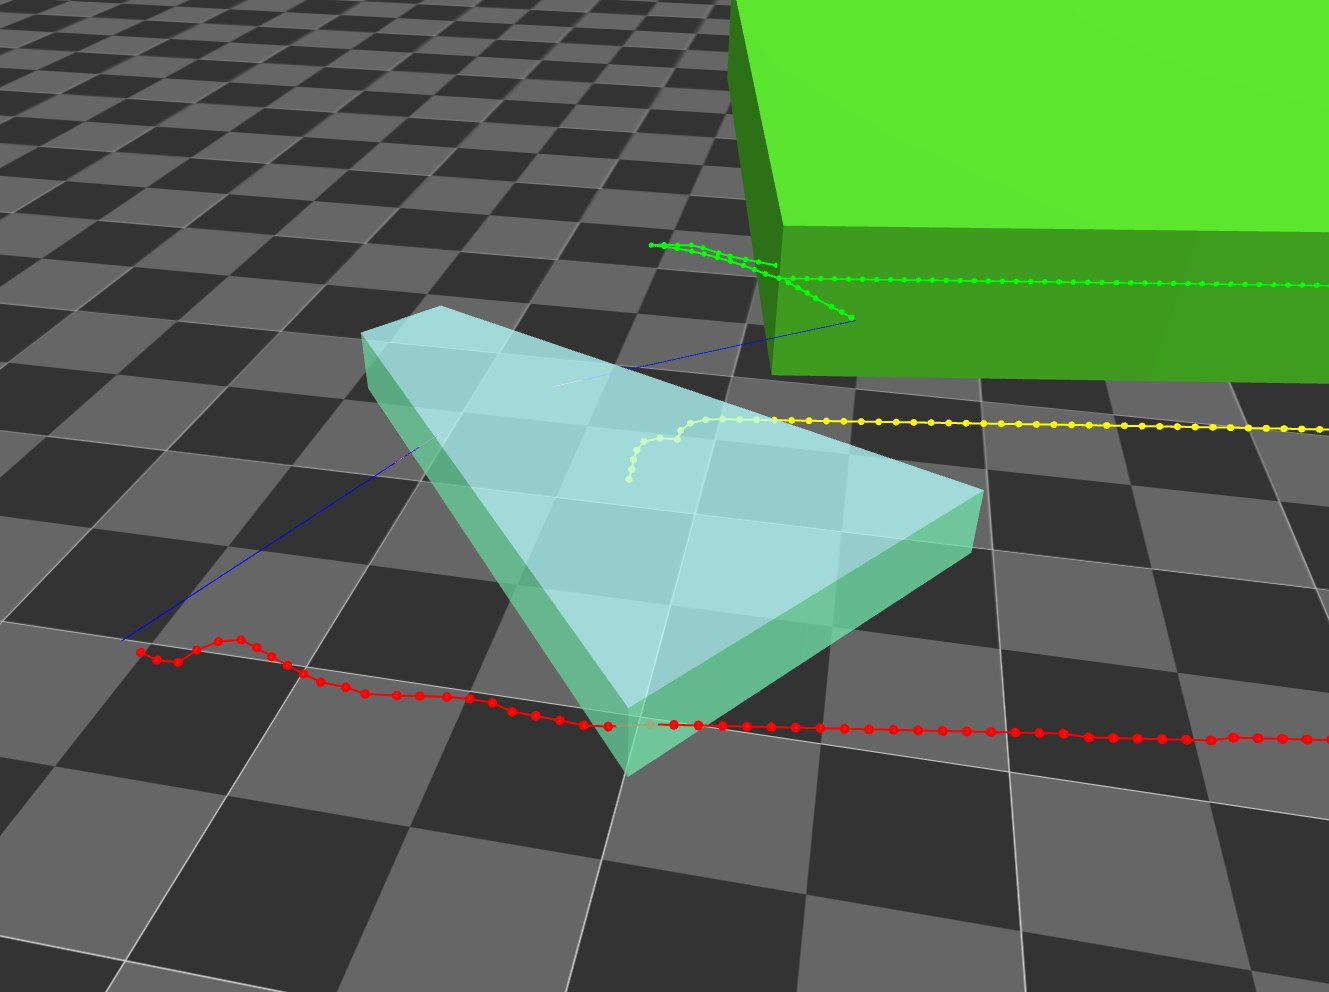
\includegraphics[width=\textwidth]{figures/retrieval/whisking}
                    \caption{\textbf{(2) Whisking}\\Moving back along the opposite side of the edge.}
                \end{figure}
            \end{column}
            \begin{column}[T]{0.48\textwidth}
                \begin{figure}[H]
                    \centering
                    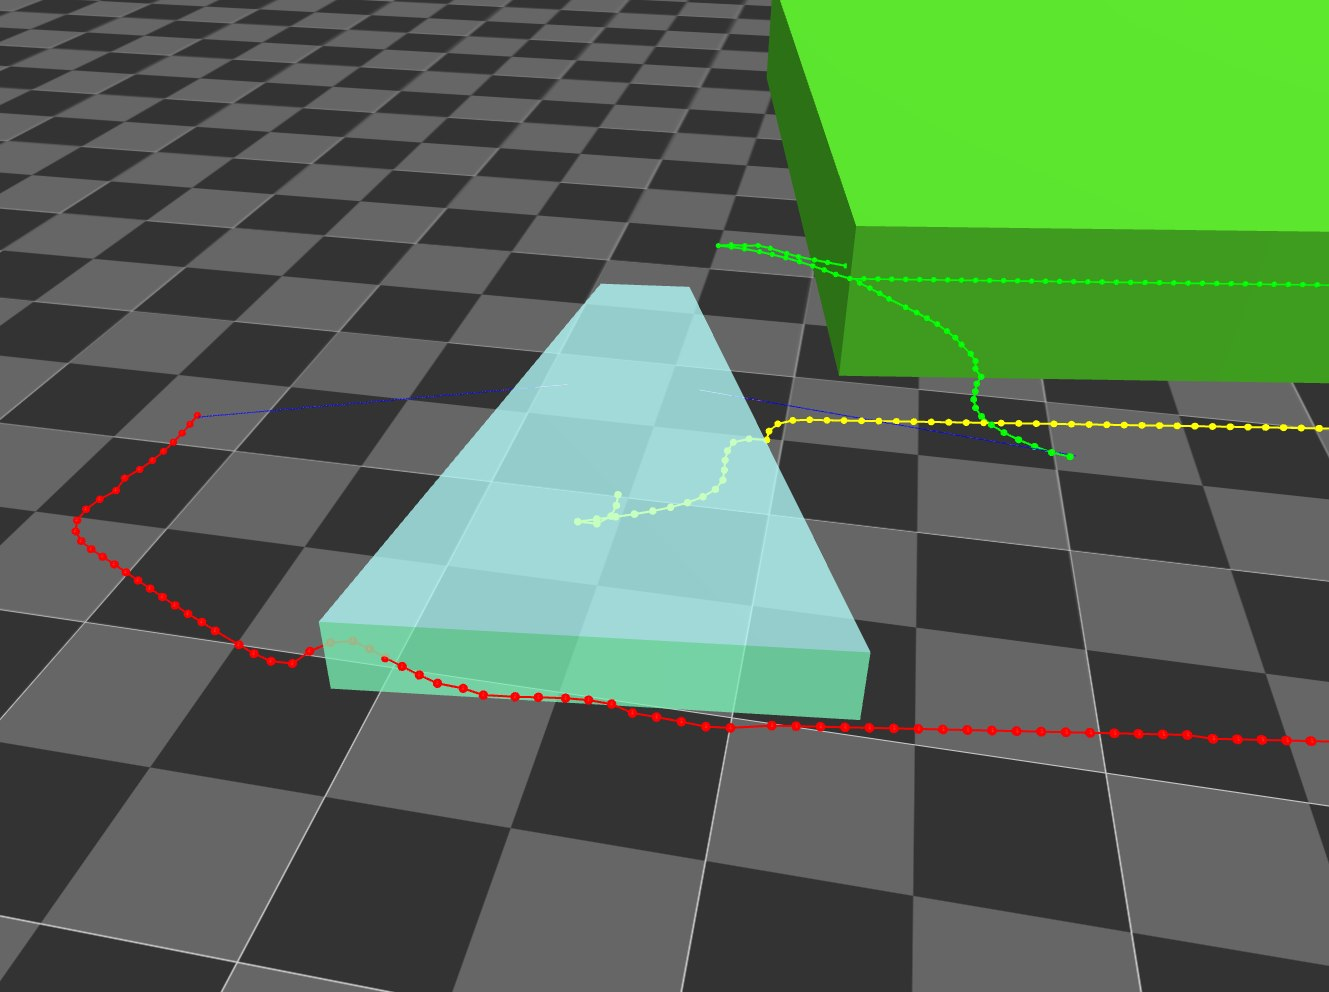
\includegraphics[width=\textwidth]{figures/retrieval/repositioning}
                    \caption{\textbf{(3.1) Repositioning}\\Assuming an optimal position for approach.}
                \end{figure}
            \end{column}
        \end{columns}
    \end{frame}
    \begin{frame}[c]{Retrieval Policy}{Final Steps}
        \begin{columns}[T,onlytextwidth]
            \begin{column}[T]{0.48\textwidth}
                \begin{figure}[H]
                    \centering
                    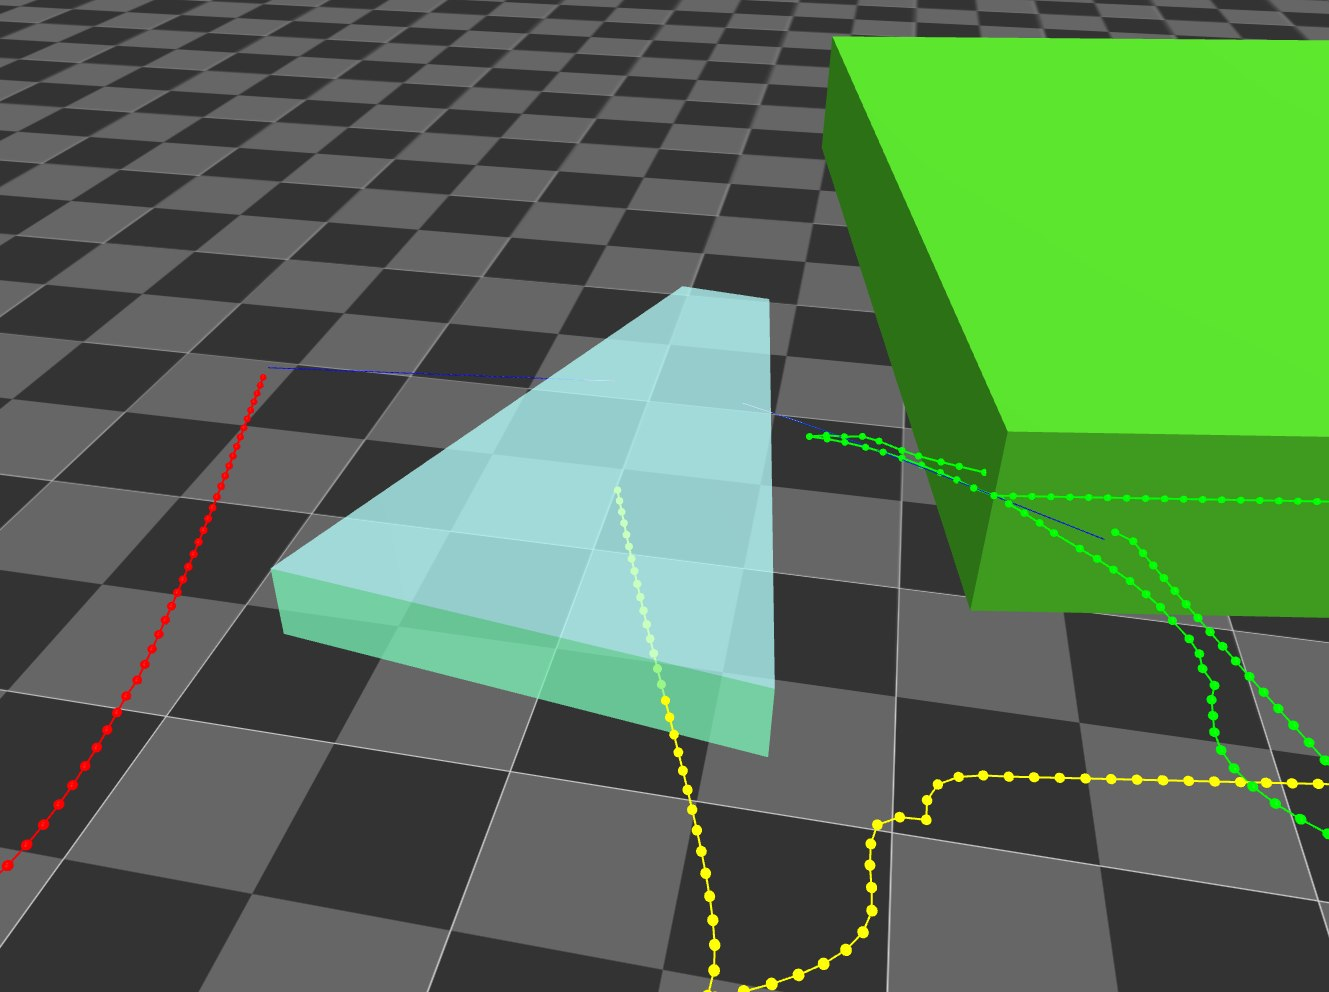
\includegraphics[width=\textwidth]{figures/retrieval/approach}
                    \caption{\textbf{(3.2) Approach}\\Moving towards the object.}
                \end{figure}
            \end{column}
            \begin{column}[T]{0.48\textwidth}
                \begin{figure}[H]
                    \centering
                    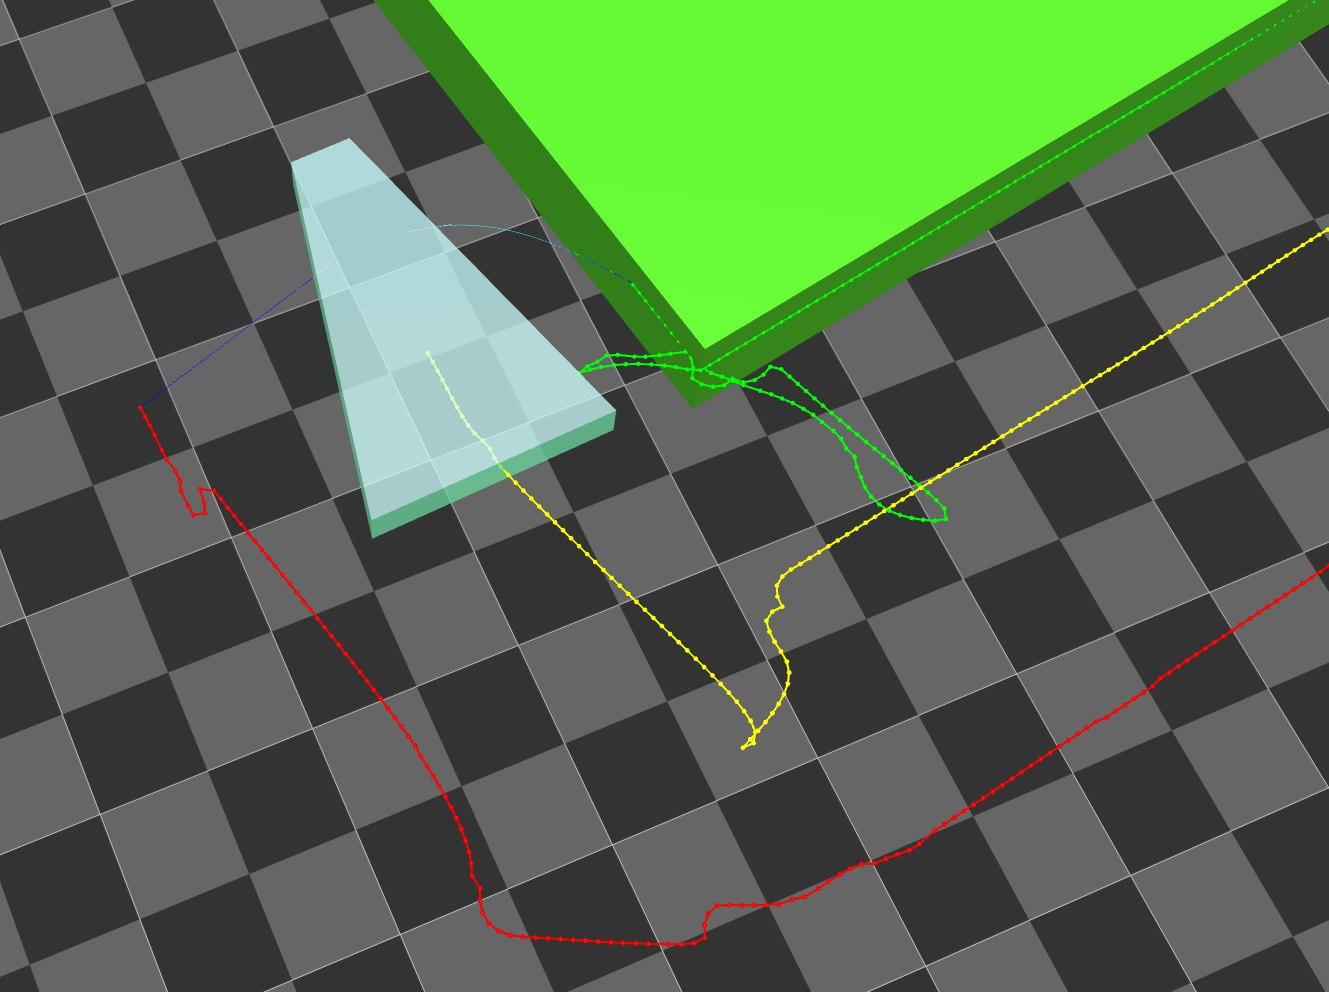
\includegraphics[width=\textwidth]{figures/retrieval/trajectory}
                    \caption{\textbf{(3.3) Transition to Swiping}\\Transferring control to the Swiping Policy.}
                \end{figure}
            \end{column}
        \end{columns}
    \end{frame}
    \begin{frame}{Retrieval Policy}{Simulation Results}
        \begin{figure}[htb]
            \centering
            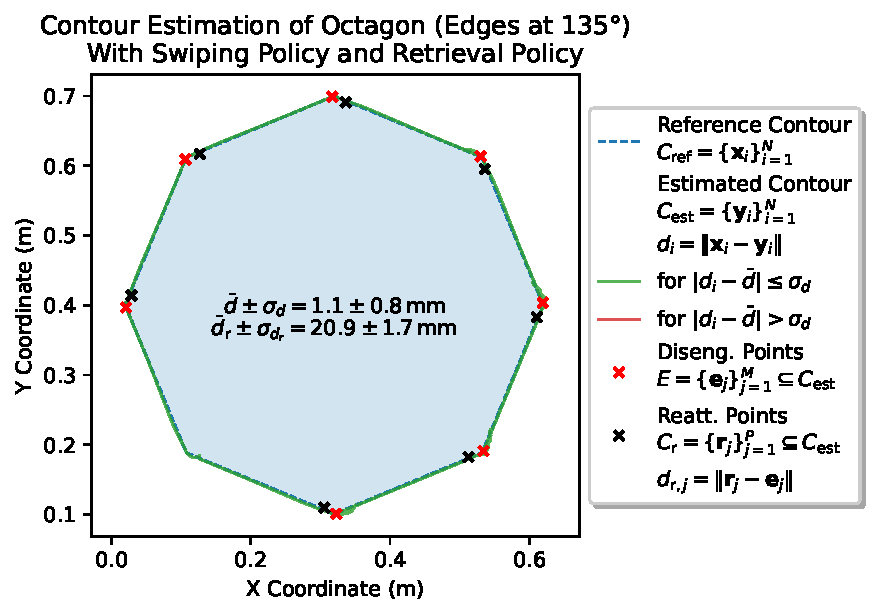
\includegraphics[width=0.7\textwidth]{figures/experiments/octagon-edges-135deg-swiping-retrieval}
        \end{figure}
    \end{frame}
    \begin{frame}{Retrieval Policy}{Simulation Results}
        \begin{figure}[htb]
            \centering
            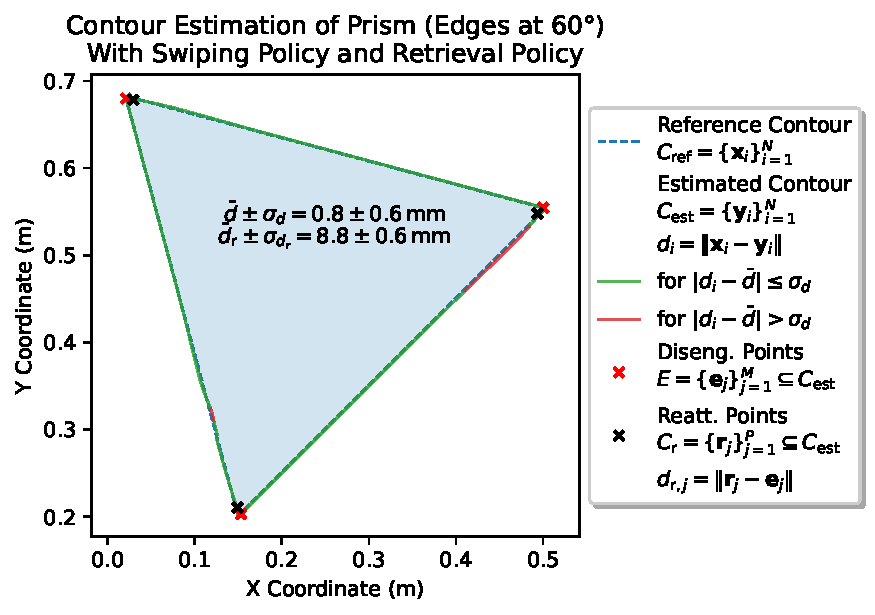
\includegraphics[width=0.7\textwidth]{figures/experiments/prism-edges-60deg-swiping-retrieval}
        \end{figure}
    \end{frame}
    \begin{frame}{Retrieval Policy}{Simulation Results}
        \begin{figure}[htb]
            \centering
            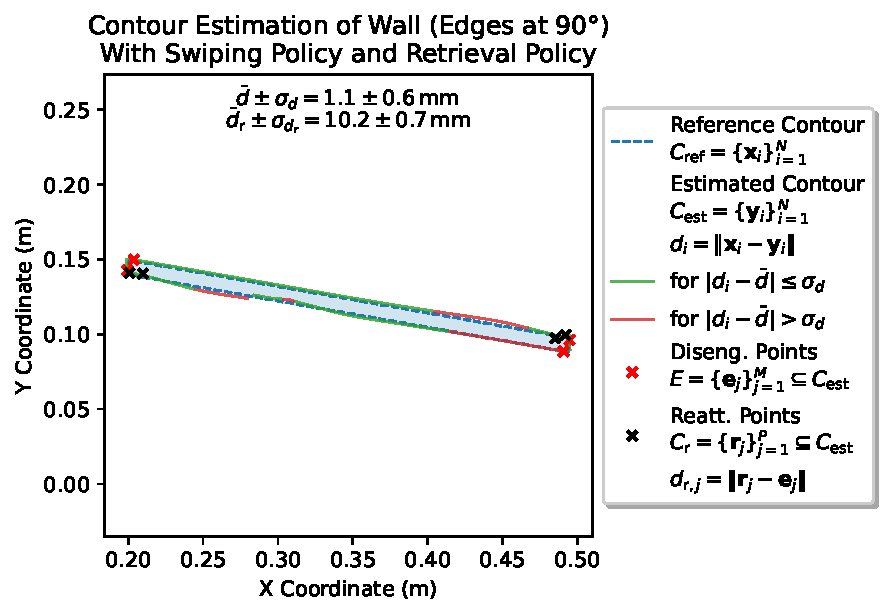
\includegraphics[width=0.7\textwidth]{figures/experiments/wall-edges-90deg-swiping-retrieval}
        \end{figure}
    \end{frame}

    \subsection{Tunneling Policy}
    \begin{frame}{Swiping Policy}{Control Algorithm}
        \begin{algorithm}[H]
            \caption{Tunneling Policy Control}
            \begin{algorithmic}[1]
                \State \(\;^{\mathrm{w}}\boldsymbol{r}_{\mathrm{tip, r}}^{t} \gets \;^{\mathrm{w}}\boldsymbol{r}^{t} + \;^{\mathrm{w}}\boldsymbol{r}_{\mathrm{r, body}} + \boldsymbol{R}_{xy}^{2}(\; ^{\mathrm{w}}\alpha_{\mathrm{r}}^{t}) \cdot \mathrm{r.defl\_model}(\delta_{\mathrm{r}}^{t})\)
                \State \(\;^{\mathrm{w}}\boldsymbol{r}_{\mathrm{tip, l}}^{t} \gets \;^{\mathrm{w}}\boldsymbol{r}^{t} + \;^{\mathrm{w}}\boldsymbol{r}_{\mathrm{l, body}} + \boldsymbol{R}_{xy}^{2}(\; ^{\mathrm{w}}\alpha_{\mathrm{l}}^{t}) \cdot \mathrm{l.defl\_model}(\delta_{\mathrm{l}}^{t})\)
                \State \colorbox{yellow!40}{\(\mathrm{midpoint\_spline.add\_keypoint}\big((\;^{\mathrm{w}}\boldsymbol{r}_{\mathrm{tip, r}}^{t} + \;^{\mathrm{w}}\boldsymbol{r}_{\mathrm{tip, l}}^{t}) / 2\big)\)}
                \State If not \(\mathrm{midpoint\_spline.has\_enough\_points}\) Then Return \(\;^{\mathrm{w}}\boldsymbol{v}^{t}\), \(\;^{\mathrm{w}}\omega^{t}\) End If
                \State
                \State \(\;^{\mathrm{w}}\boldsymbol{\tau}_{\mathrm{spline}}^{t} \gets \mathrm{midpoint\_spline}(u\mathord{=}1) - \mathrm{midpoint\_spline}(u\mathord{=}0)\)
                \State \(\;^{\mathrm{w}}\boldsymbol{n}_{\mathrm{spline}}^{t} \gets \boldsymbol{R}_{xy}^{2}(\pi/2 \cdot orient_\mathrm{r}^t)\cdot\;^{\mathrm{w}}\boldsymbol{\tau}_{\mathrm{spline}}^{t}\)
                \State \colorbox{cyan!40}{\(\;^{\mathrm{w}}\theta_{\mathrm{spline}}^{t} \gets \mathrm{arctan2}(\;^{\mathrm{w}}\boldsymbol{\tau}_{\mathrm{spline}}^{t})\)}
                \State \(\mathrm{pull_{total}} \gets \mathrm{clip}\big(\frac{\delta_{\mathrm{r}}^{t} - \delta_{\mathrm{r, target}}}{\delta_{\mathrm{r, target}}} - \frac{\delta_{\mathrm{l}}^{t} - \delta_{\mathrm{l, target}}}{\delta_{\mathrm{l, target}}},\mathrm{\min}\mathord{=}-1, \mathrm{\max}\mathord{=}1\big)\)
                \State \colorbox{green!40}{\(\;^{\mathrm{w}}\boldsymbol{r}^{t+1} \gets \;^{\mathrm{w}}\boldsymbol{r}^{t} + \;^{\mathrm{w}}\boldsymbol{\tau}_{\mathrm{spline}}^{t} + \mathrm{pull_{total}}/2 \cdot \;^{\mathrm{w}}\boldsymbol{n}_{\mathrm{spline}}^{t}\)}
                \State \((\;^{\mathrm{w}}\boldsymbol{v}^{t+1}, \;^{\mathrm{w}}\omega^{t+1}) \gets steer\_body(\;^{\mathrm{w}}\boldsymbol{r}^{t+1},\;^{\mathrm{w}}\theta_{\mathrm{spline}}^{t})\)
                \State Return \(\;^{\mathrm{w}}\boldsymbol{v}^{t+1}, \;^{\mathrm{w}}\omega^{t+1}\)
            \end{algorithmic}
        \end{algorithm}
    \end{frame}
    \begin{frame}{Tunneling Policy}{Simulation Results}
        \begin{figure}[htb]
            \centering
            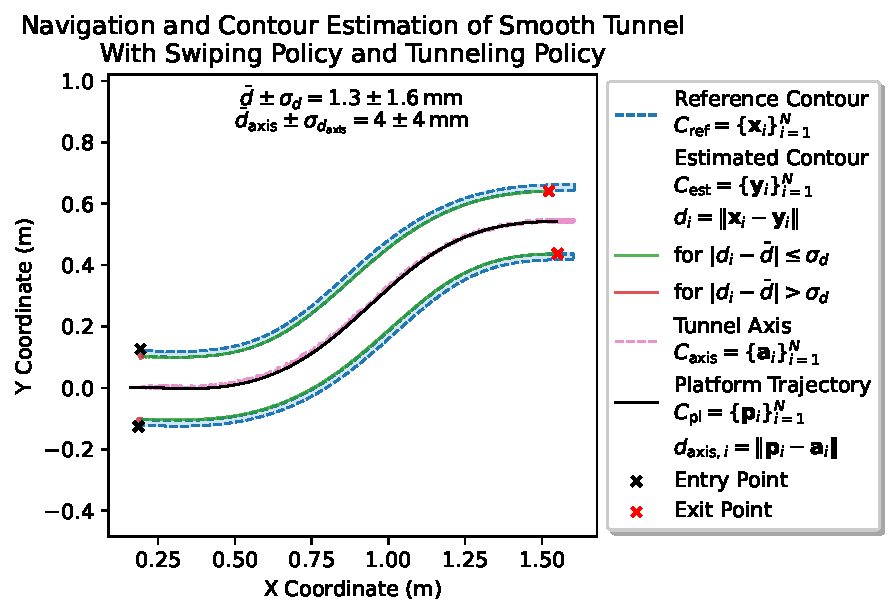
\includegraphics[width=0.7\textwidth]{figures/experiments/smooth-tunnel-swiping-tunneling}
        \end{figure}
    \end{frame}
    \begin{frame}{Tunneling Policy}{Simulation Results}
        \begin{figure}[htb]
            \centering
            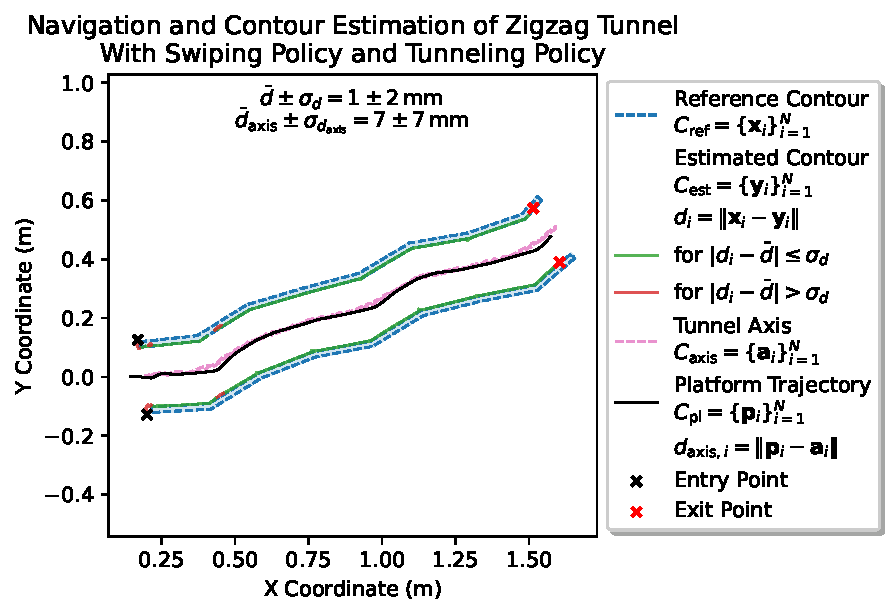
\includegraphics[width=0.7\textwidth]{figures/experiments/zigzag-tunnel-swiping-tunneling}
        \end{figure}
    \end{frame}
    \begin{frame}{Tunneling Policy}{Simulation Results}
        \begin{figure}[htb]
            \centering
            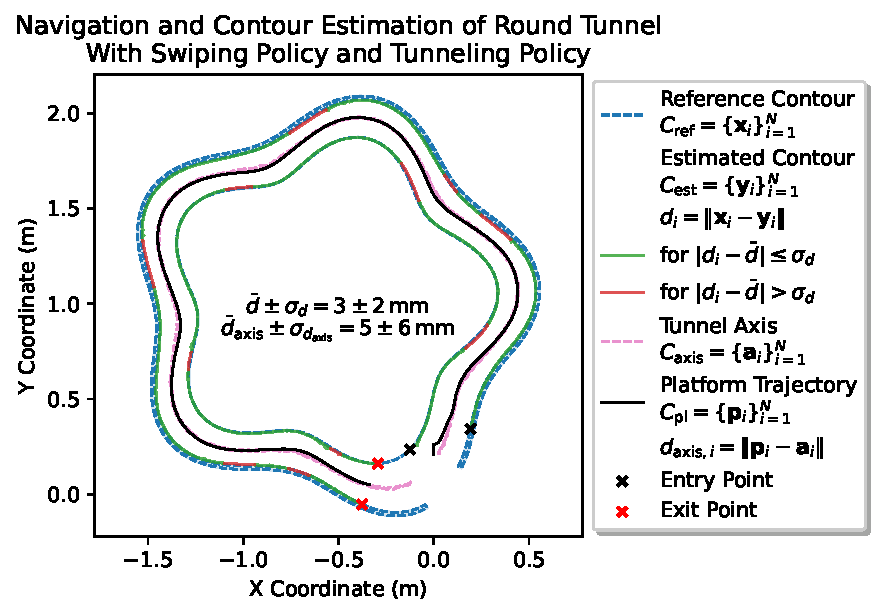
\includegraphics[width=0.7\textwidth]{figures/experiments/round-tunnel-swiping-tunneling}
        \end{figure}
    \end{frame}

    \subsection{Governing Policy}
    \begin{frame}{Governing Policy}{Finite State Machine}
        \begin{figure}[H]
            \centering
            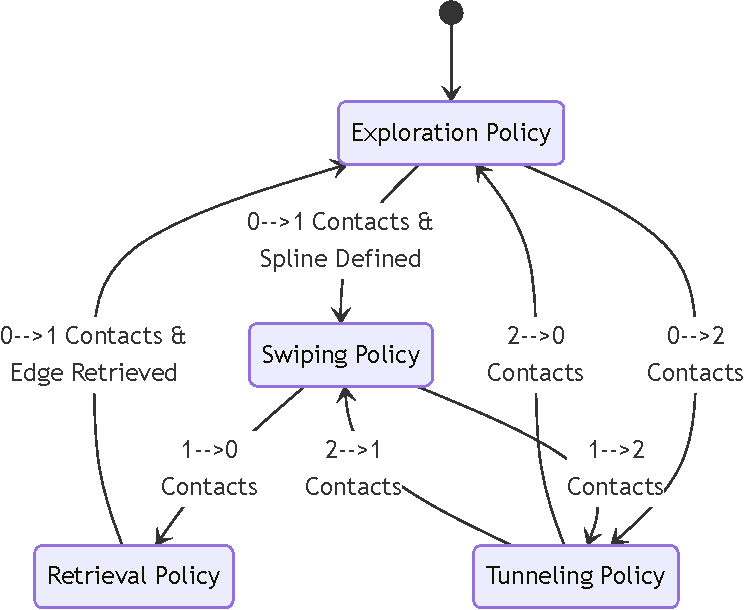
\includegraphics[width=0.6\textwidth]{figures/fsm}
            \caption{FSM diagram of the whisker control system.}
        \end{figure}
    \end{frame}


    \section{Infrastructure}
    \begin{frame}{Infrastructure}{System Overview}
        \begin{figure}[H]
            \centering
            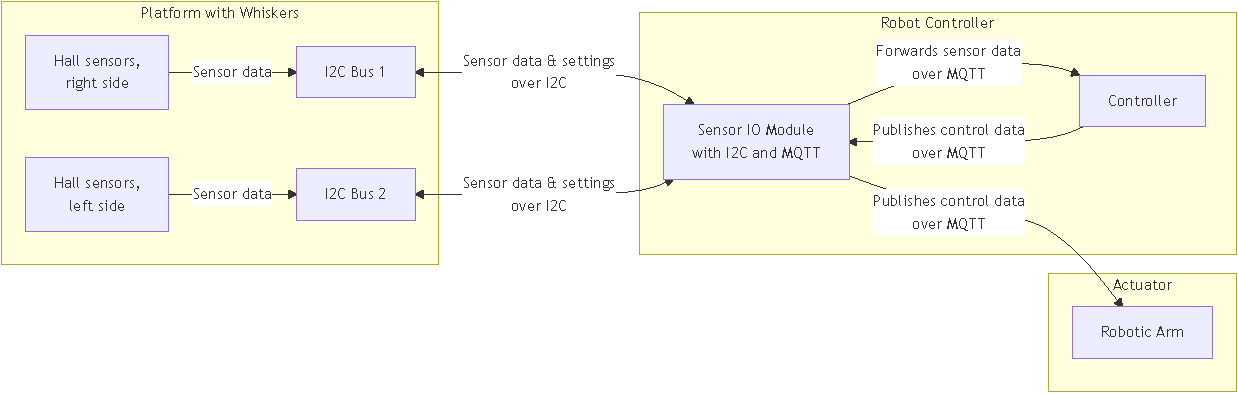
\includegraphics[width=\textwidth]{figures/infrastructure-overview}
            \caption{Data flow in the system infrastructure.}
        \end{figure}
    \end{frame}

    \begin{frame}{Infrastructure}{Robot Controller Overview}
        \begin{figure}[H]
            \centering
            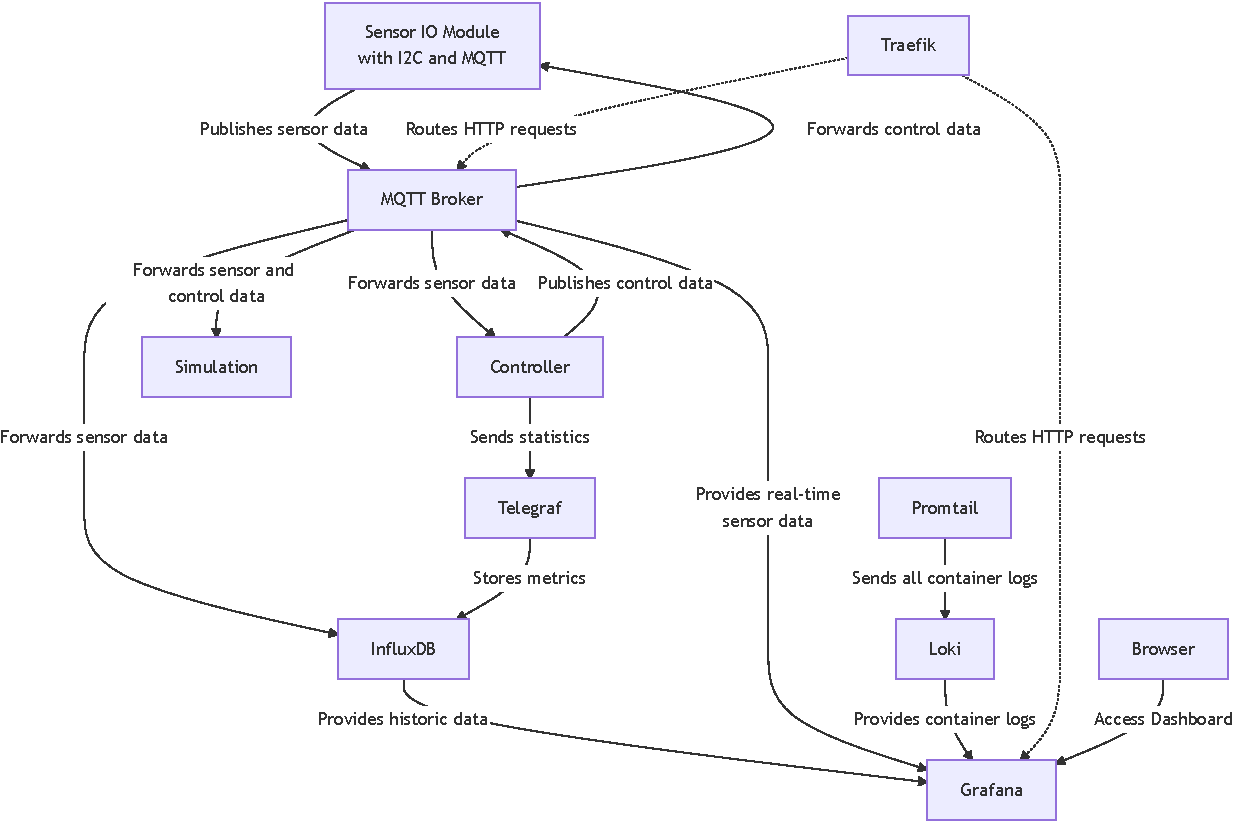
\includegraphics[height=0.75\textheight]{figures/infrastructure-robot-controller}
            \caption{Data flow in the robot controller infrastructure.}
        \end{figure}
    \end{frame}

    \begin{frame}{Infrastructure}{Data Visualization}
        \begin{figure}[H]
            \centering
            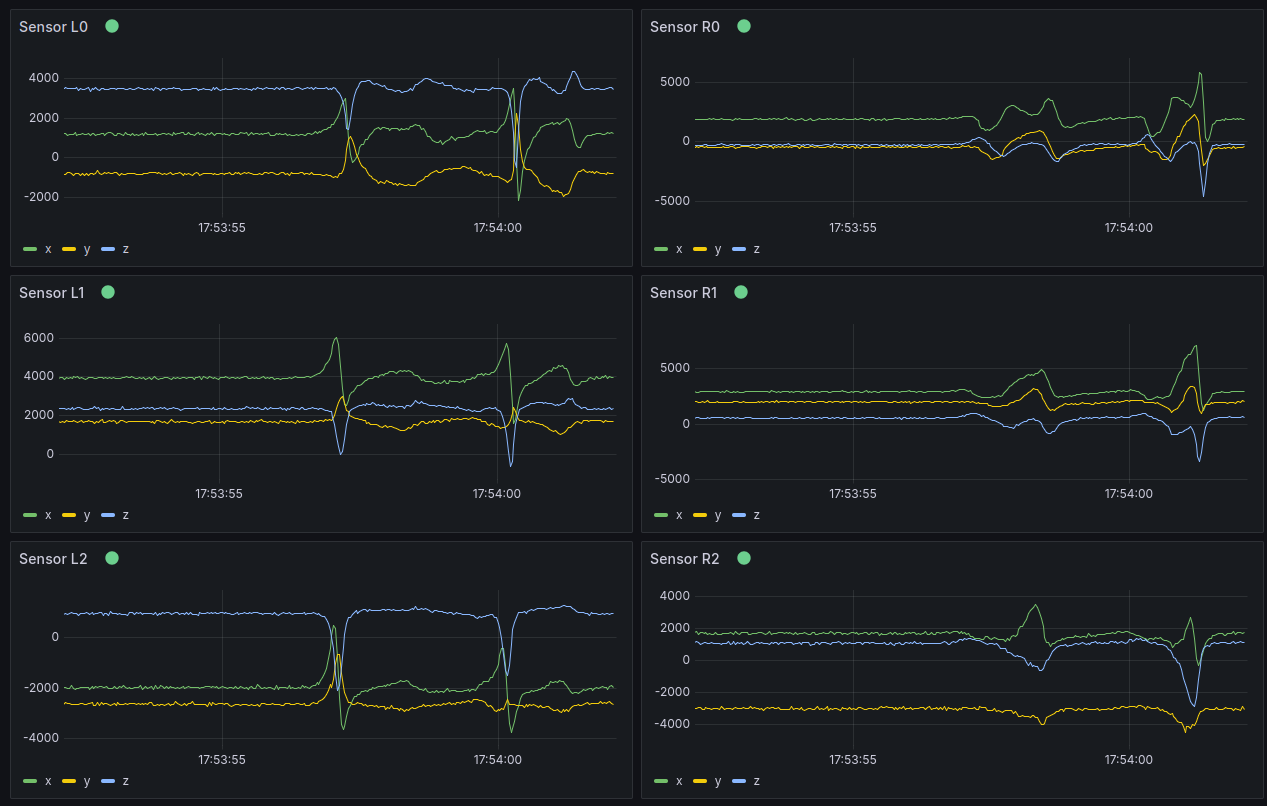
\includegraphics[width=0.7\textwidth]{figures/grafana}
            \caption{Sensor data visualization in real time using Grafana.}
        \end{figure}
    \end{frame}


    \section{Future Work}
    \begin{frame}{Future Work}
        \begin{itemize}
            \item Testing of the whisker control system with the Franka Emika Panda robotic arm
            \item Addition of more whiskers to each side of the platform
            \item Active exploration of unstructured environments
            \item SLAM for navigation in cluttered environments
            \item Integration of the whiskers into the robotic rat
        \end{itemize}
    \end{frame}


    \section{Conclusion}
    \begin{frame}{Conclusion}
        \begin{columns}[T,onlytextwidth]
            \begin{column}[T]{0.6\textwidth}
                \begin{minipage}[c][.8\textheight][c]{\linewidth}
                    \begin{enumerate}
                        \item A \textbf{whisker array platform} for active tactile exploration was designed and assembled
                        \item Control algorithms were implemented for:
                        \begin{itemize}
                            \item Contour reconstruction
                            \item \textbf{Object retrieval}
                            \item \textbf{Navigation in tunnels}
                        \end{itemize}
                        \item A \textbf{test framework with physics simulation} was developed for the whisker control system
                        \item A \textbf{system infrastructure} was developed for real-time sensor data visualization and evaluation
                    \end{enumerate}
                \end{minipage}
            \end{column}
            \begin{column}[T]{0.4\textwidth}
                \begin{figure}[H]
                    \centering
                    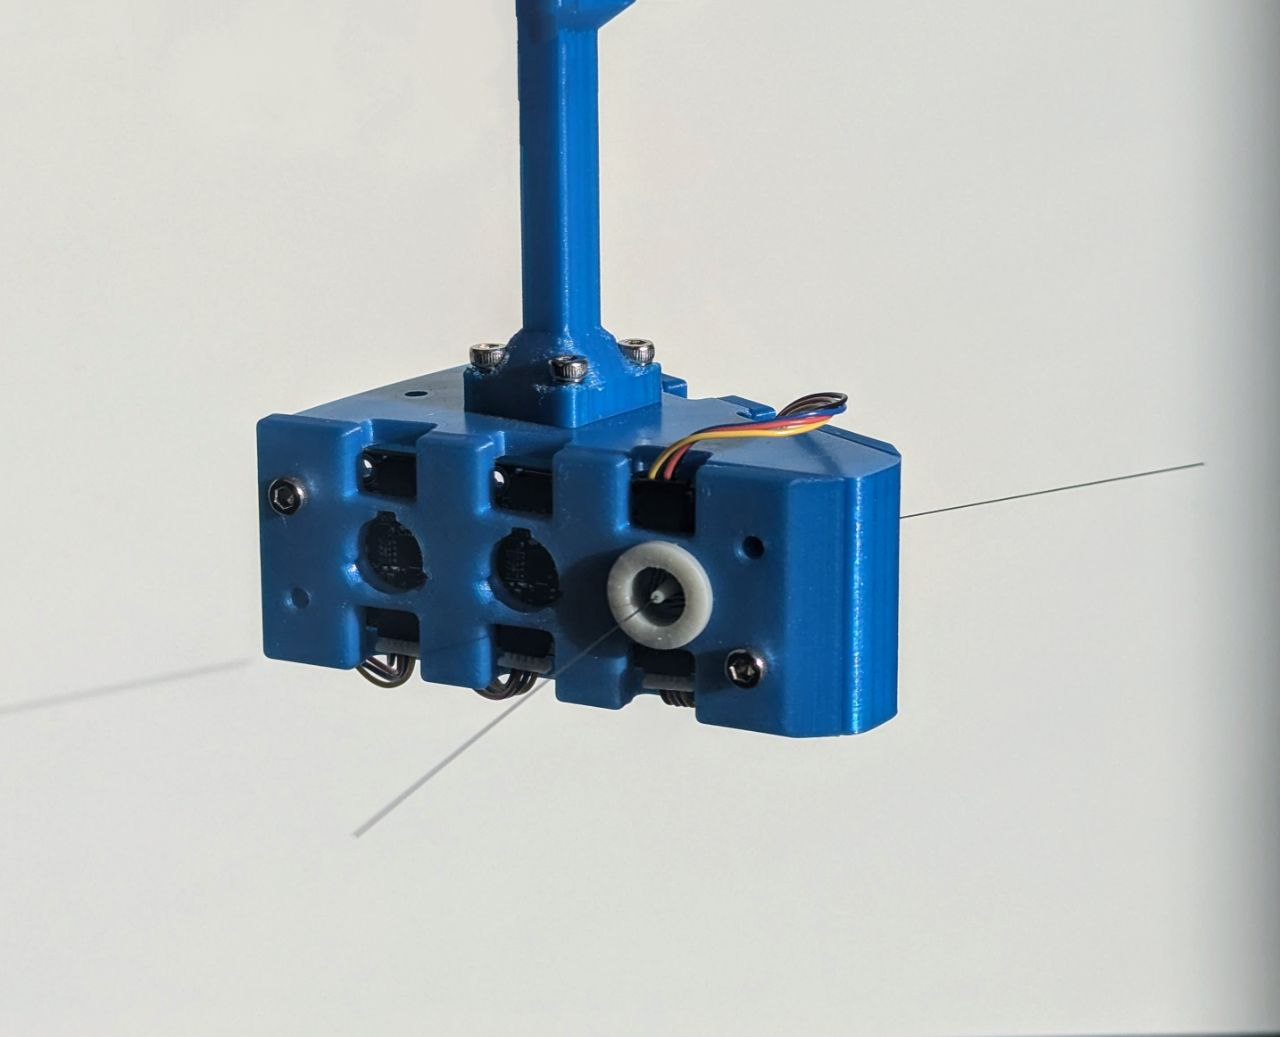
\includegraphics[width=0.7\textwidth]{figures/platform-two-whiskers}
                \end{figure}
                \vskip-0.5cm
                \begin{figure}[H]
                    \centering
                    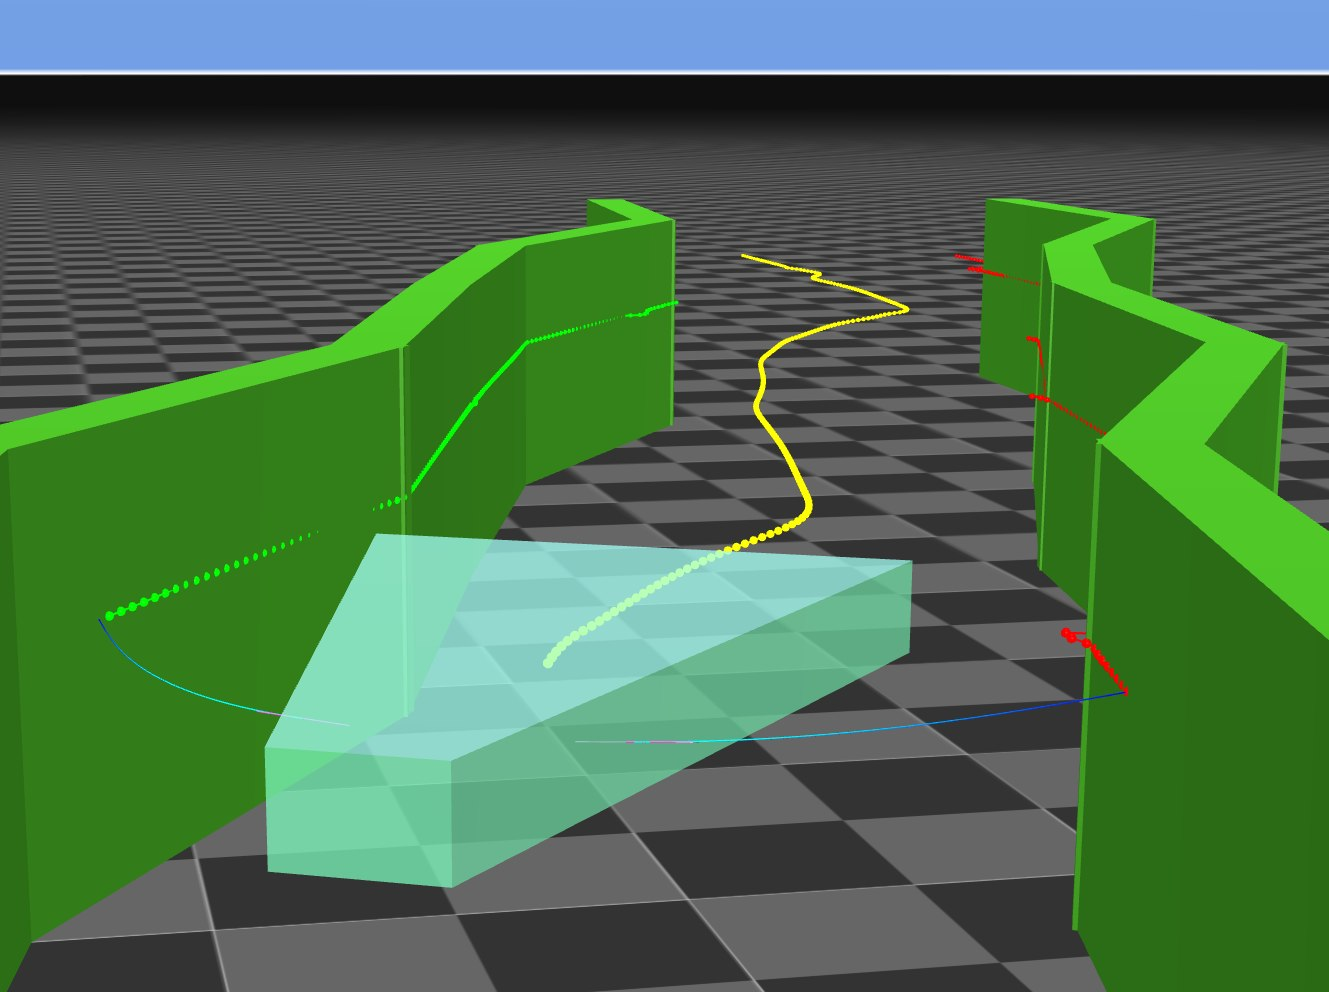
\includegraphics[width=0.7\textwidth]{figures/platform-in-tunnel}
                \end{figure}
            \end{column}
        \end{columns}
    \end{frame}


    \AIRbeamerSetFooterText{References}
    \begin{frame}[allowframebreaks]{References}
        %\sloppy% "Word"-like typesetting in order to improve breaking lines with long URLs/DOIs
        \printbibliography[heading=none]
    \end{frame}%

    \AIRbeamerTitlePageStudentThesis%

\end{document}%
